\documentclass[12pt]{report}

\usepackage{algorithm}
\usepackage{algpseudocodex}
\usepackage{amsmath}
\usepackage{amssymb}
\usepackage[toc,page]{appendix}
\usepackage{blkarray}
\usepackage{float}
\usepackage[total={6.25in, 8.50in}]{geometry}
\usepackage{graphicx}
\usepackage[hidelinks]{hyperref}
\usepackage{longtable}
\usepackage{mathtools}
\usepackage{natbib}
\usepackage{parskip}
\usepackage{pgfplots}
\usepackage{pgfplotstable}
\usepackage{setspace}
\usepackage{subcaption}
\usepackage{tikz}

\pgfplotsset{compat=1.18}

\usetikzlibrary{positioning}

\title{DamathZero: Learning How to Play Damath through Self-Play}

\author{Daniel David N. Bador \\ Brymer Bernard R. Meneses}

\date{\today}

\doublespacing
\begin{document}

\maketitle

\chapter*{Acknowledgements}
\addcontentsline{toc}{chapter}{Acknowledgement}

The authors thank Professor Lee Javellana for his patience, guidance, and support throughout this study.  We also thank Mr. Basanes for voluntarily imparting his knowledge in the game of Damath. This study would not be possible without his expertise.

In addition, we would like to thank our family. The authors thank Mr. Bernard and Mrs. Merryl Meneses for their constant support and for leading us to communicate with Mr. Basanes. We also thank Mr. David and Mrs. Virna Bador for their constant and everlasting support throughout our time in college.

Special thanks are due to our friends who made our undergraduate years bearable and fun, Joana Mariel Santiago, Hannah Kathrina Ramos, Charrie Anne Nacor, Lester Ignacio, Andre Bryant Bagalso, Grandemir Baysa-Pee and Zed De Guzman.

% We also thank Alpha Phi Omega - Gamma Pi Chapter for 

% We also thank Common Ground and their staff for being a good host throughout our studies. We would not be able to work comfortably in our study without the warm ambiance and ample amount of coffee they provide to us every night and day.

Lastly, we also thank the University of the Philippines-Baguio, for molding us to what we are today. As scholars of the Philippines, the university has shaped us to be as sharp and critical as we are now.


% I would like to thank the members of my thesis committee for their help in preparation of this work – Niles Caulder, without whom I would have been doomed to never complete it, Kimiyo Hoshi, who helped to shed new light on many of my ideas, Pamela Isley, with whom I often disagree but who inspires me to be better, Raymond Palmer, who had no small part to play in the formation of the idea, and Kent Nelson, who always
% had golden advice.

% Special thanks are due to the friends and colleagues who made this work possible. Jimmy Olsen and Pete Ross were invaluable both as friends and as sounding boards for some of my more outlandish ideas. Jack Knight, who I met only briefly, was a major influence, and I’m glad we were able to help each other.

% The author gratefully acknowledges the support for this work offered by S.T.A.R. Laboratories under grant award number 3X29YZ4A, and by the Theodore S. Kord Fellowship. Any views and conclusions contained herein are those of the author, and do not necessarily represent the official positions, express or implied, of the funders.
\begin{abstract}
\addcontentsline{toc}{chapter}{Abstract}

Damath is an educational board game that is commonly played throughout the Philippines. It is also used as a competitive game for all levels of education with different variations. This paper uses the AlphaZero framework to train a model of the Vision Transformer with Jumbo CLS token architecture and the C++ front-end of PyTorch to learn how to play integer Damath through self-play. The model was able to develop its own strategies without prior human knowledge of the game except for the rules of Damath. The researchers were able to produce five different versions of the best model for twenty iterations over 2.5 days on the cloud with a computer that has 515673MiB of RAM, an AMD Ryzen Threadripper PRO 3975WX CPU with 32 cores at 3.5000 GHz clock speed, and an NVIDIA GeForce RTX 4090 GPU on an Ubuntu 25.04 Linux Virtual Machine. The fifth and final version of the model beats all of the previous versions of the model and was also able to beat an expert Damath player for three out of ten games. However, the model exhibits strong-early game but weak middle-to-late game competence which is due to the short training time and computatational resources.

\end{abstract}

\tableofcontents

\listoffigures
\listoftables
\listofalgorithms

\chapter{Introduction}

Games like Chess, Shogi, Go, and Checkers are games in which each player has perfect information regarding the state of the game. According to \cite{MYCIELSKI199241}, perfect information means that there is no hidden information between the players, each time only one of the player moves, that the game depends only on their choices, every player remembers the past, and in principle they know all the possible futures of the game.

Throughout history, these games have been benchmarks for intelligence. That is why numerous attempts have been made to beat humans in these games. DeepBlue is the first artificial intelligence to defeat a grandmaster in the game of chess in a professional setting \cite{hsu2002behind}.

\section{Background of the Study}

Artificial intelligence (AI) has made significant strides in recent years, achieving groundbreaking results in areas previously thought to require human intuition and expertise. Notable among these advancements is AlphaZero, an AI developed by DeepMind that has demonstrated an ability to master complex games such as Chess, Go, and Shogi \cite{silver2017masteringchessshogiselfplay}. By employing deep reinforcement learning and self-play, AlphaZero has set new standards in artificial intelligence by learning game strategies autonomously without any human input beyond the basicwrules of each game. This breakthrough has inspired researchers to explore applications of AlphaZero’s learning model in diverse domains.

One such potential application is in the game of Damath. Damath is a Filipino educational board gamewthat combines the principles of mathematics with the strategic nature of a board game. The game is similar to Checkers but integrates mathematical operations into each move, requiring players to use mathematical strategies along with spatial and strategic thinking. As a tool for enhancing students' mathematical and analytical skills, Damath has become popular in Philippine schools. 

Applying AlphaZero to Damath presents an opportunity not only to advance AI applications in local games but also to explore new approaches to educational AI, contributing to both the fields of AI research and educational technology.

The original AlphaZero paper makes use of Convolutional Neural Networks  particularly the ResNet architecture to develop a competitive model for games such as Chess, Shogi, and Go. However, recent advances in Computer Vision, have shown that Vision Transformers can beat Convolutional Neural Networks (\cite{dosovitskiy2021imageworth16x16words}), which inspired the researchers to determine the feasibility of this architecture and see if they can train such model to become competitive in the game of Damath.

\section{Problem Statement}

To the extent of the researchers' knowledge, most programs that play Damath rely on programmed rules or decision trees that do not fully explore the strategic potential of the game. This limitation results in AI opponents that are relatively easy to predict and exploit, reducing the educational value and engagement level for players. An AlphaZero-based model could provide a self-learning AI capable of adapting to the unique strategies and mathematical complexities of Damath, resulting in a more challenging and dynamic opponent.

This research explores the feasibility of training a model with a Vision Transformer architecture using the AlphaZero framework, and determine if it can learn various strategies in the game of Damath without prior human knowledge beyond the rules of the game. 

\section{Objectives of the Study}

The primary objective of this study is to develop and evaluate an AlphaZero-based AI model tailored to the game of Damath, more specifically integer Damath. Specific objectives include:
\begin{enumerate}
    \item  To train a model that is proficient in the game of Damath, without prior human knowledge.
    \item To evaluate the performance of the AlphaZero-based Damath AI by testing it against human players and against itself.
    \item To analyze the AI’s learning process and behavior, examining whether it can effectively learn and adapt to optimal Damath strategies without external guidance.
    % \item To assess the educational impact of the AlphaZero-based Damath AI on players, particularly in terms of enhancing their mathematical and strategic thinking abilities.
\end{enumerate}

\section{Significance of the Study}

The significance of this study lies in its potential contributions to both artificial intelligence research and educational gaming. From a technical perspective, adapting AlphaZero to a game like Damath requires innovations in handling mathematical operations as part of the AI’s decision-making process, a feature not present in typical board games like Chess or Go. Success in this endeavor could provide insights into the adaptability of AlphaZero in various educational and non-standard game environments, offering a model for future AI research in educational games.

From an educational perspective, this study could improve the effectiveness of Damath as a teaching tool, offering students a more challenging and interactive experience. An advanced AI opponent could encourage students to think critically, refine their strategies, and improve their mathematical skills, contributing to a deeper understanding and appreciation of mathematics through play.

\section{Scope and Limitations}

This study will focus on adapting the AlphaZero framework specifically to the rules and gameplay of Damath. There are many variations to the game of Damath, this study will only focus on integer Damath. Additionally, given computational constraints, the model's training process may be limited to a defined number of games or iterations. Limitations of the study include computational resources, as AlphaZero requires significant processing power for optimal training results.

\section{Organization of the Study}

The succeeding chapters of this study are organized as follows:
\begin{itemize}
    \item Chapter 2: Preliminaries – Discusses previous works and studies on AlphaZero and Damath.
    \item Chapter 3: Methodology – Details the approach, model design, and implementation process for developing the AlphaZero-based Damath AI.
    \item Chapter 4: Results and Discussion – Presents and analyzes the results of the AI’s performance.
    \item Chapter 5: Conclusion and Recommendations – Summarizes the study’s findings and suggests areas for future research.
\end{itemize}

In the following chapters, we delve deeper into the research questions and review the current state of AI applications in games, setting the foundation for this investigation into AlphaZero’s applicability to Damath.
\chapter{Preliminaries}

This chapter reviews the theoretical and empirical literature surrounding the core concepts of this research, namely AlphaZero, and its core components, the Monte-Carlo Tree Search, a deep neural network and reinforcement learning.

\section{Mathematical Concepts}

A set is a well-defined collection of objects (\cite{diestel2024graph}).

A function $f: X \to Y$ is a subset of $X \times Y$ such that for each $x \in X$, there is a unique $y \in Y$ such that $(x, y) $ is in the subset (\cite{thielman1953definition}).

The derivative of a function denoted by $f'(x)$ is defined by Equation \ref{eq:derivative} (\cite{kalanov2019definition}).

\begin{equation}
    f'(x) = \frac{df}{dx} = \lim_{h \to 0} \frac{f(x+h) - f(x)}{h}
    \label{eq:derivative}
\end{equation}

The partial derivative of a multivariable function $f(x_1, x_2, \ldots, x_n)$ with respect to $x_i$ for $1 \le i \le n$ denoted by $\dfrac{\partial f}{\partial x_i}$ is defined by Equation \ref{eq:partial-derivative} (\cite{widder2012advanced}).

\begin{equation}
    \frac{df}{\partial x_i} = \lim_{h \to 0} \frac{f(x_1, x_2, \ldots, x_i + h, \ldots, x_n) - f(x_1, x_2, \ldots, x_i, \ldots, x_n)}{h}
    \label{eq:partial-derivative}
\end{equation}

The gradient $\nabla$ of a multivariable function $f(x_1, x_2, \ldots, x_n)$ is defined by Equation \ref{eq:gradient} (\cite{calder2020calculus}). The gradient descent of a function $-\nabla f$ at point $p$ points to the direction for which $(p, f(p))$ has the highest descent.

\begin{equation}
    \nabla f = \left[\dfrac{\partial f}{\partial x_{1}}, \dfrac{\partial f}{\partial x_{2}}, \dfrac{\partial f}{\partial x_{3}}, \ldots, \dfrac{\partial f}{\partial x_{n}} \right]^T
    \label{eq:gradient}
\end{equation}

A graph $G$ is a pair of two sets $(V, E)$ where $V$ is a set whose elements are called vertices, and $E$ is the set of unordered pairs $\{v_i, v_j\}$ for any connected vertices $v_i, v_j \in V$, whose elements are called edges (\cite{diestel2024graph}).

\begin{figure}[htb]
    \centering
    \begin{subfigure}{0.4\textwidth}
        \centering
        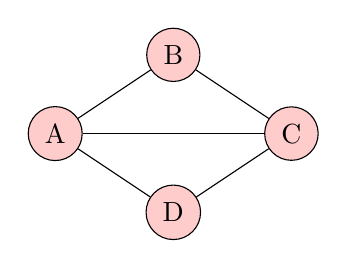
\begin{tikzpicture}
            \node[circle, draw, fill=red!20] (A) at (0, 1) {A};
            \node[circle, draw, fill=red!20] (B) at (1.5, 2) {B};
            \node[circle, draw, fill=red!20] (C) at (3, 1) {C};
            \node[circle, draw, fill=red!20] (D) at (1.5, 0) {D};
        
            \draw (A) -- (B);
            \draw (B) -- (C);
            \draw (C) -- (D);
            \draw (D) -- (A);
            \draw (A) -- (C);
        \end{tikzpicture}
        \caption{Undirected Graph}
        \label{fig:undirected-graph}
    \end{subfigure}
    \qquad
    \begin{subfigure}{0.4\textwidth}
        \centering
        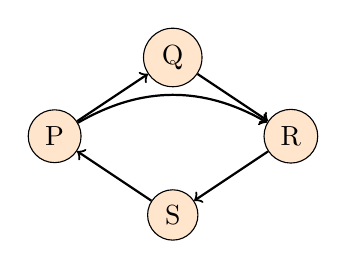
\begin{tikzpicture}
            \node[circle, draw, fill=orange!20] (P) at (5, 1) {P};
            \node[circle, draw, fill=orange!20] (Q) at (6.5, 2) {Q};
            \node[circle, draw, fill=orange!20] (R) at (8, 1) {R};
            \node[circle, draw, fill=orange!20] (S) at (6.5, 0) {S};
        
            \draw[->, thick] (P) -- (Q);
            \draw[->, thick] (Q) -- (R);
            \draw[->, thick] (R) -- (S);
            \draw[->, thick] (S) -- (P);
            \draw[->, thick] (P) to[bend left] (R);
        \end{tikzpicture}
        \caption{Directed Graph}
        \label{fig:directed-graph}
    \end{subfigure}
    \caption{Examples of Graph}
\end{figure}

A graph is said to be undirected if the edges are unordered as shown in Figure \ref{fig:undirected-graph}. That is, for all $\{v_i, v_j\} \in E, \{v_j, v_i\}\neq \{v_j, v_i\}$. Otherwise, it is called a directed graph as shown in Figure \ref{fig:directed-graph} (\cite{diestel2024graph}).

A graph is connected if for any two vertices $v_i, v_j \in V$, there exists at least one path connecting $v_i$ and $v_i$ (\cite{diestel2024graph}).

A walk is a sequence of vertices $v_1, v_2, \ldots, v_k \in V$ such that $\{v_i, v_{i+1}\} \in E$ for $1 \le i \le k$. A path is a walk with distinct vertices and edges as shown in Figure \ref{fig:path}. A cycle is a walk that starts and ends on the same vertex, it also has distinct vertices and edges with the exception of the last vertex as shown if Figure \ref{fig:cycle}. If a graph does not have a cycle, then it is called acyclic (\cite{diestel2024graph}).

\begin{figure}[htb]
    \centering
    \begin{subfigure}{0.4\textwidth}
        \centering
        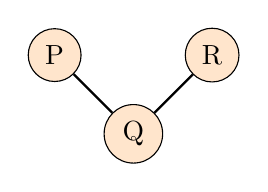
\begin{tikzpicture}
            \node[circle, draw, fill=orange!20] (P1) at (5, -4) {P};
            \node[circle, draw, fill=orange!20] (P2) at (6, -5) {Q};
            \node[circle, draw, fill=orange!20] (P3) at (7, -4) {R};
            \draw[thick] (P1) -- (P2) -- (P3);
        \end{tikzpicture}
        \caption{Path}
        \label{fig:path}
    \end{subfigure}
    \qquad
    \begin{subfigure}{0.4\textwidth}
        \centering
        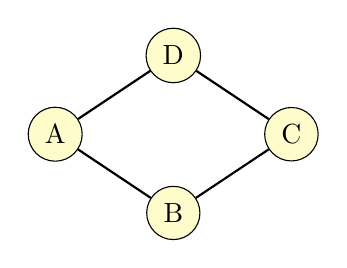
\begin{tikzpicture}
            \node[circle, draw, fill=yellow!20] (C1) at (0, -4) {A};
            \node[circle, draw, fill=yellow!20] (C2) at (1.5, -5) {B};
            \node[circle, draw, fill=yellow!20] (C3) at (3, -4) {C};
            \node[circle, draw, fill=yellow!20] (C4) at (1.5, -3) {D};
            \draw[thick] (C1) -- (C2) -- (C3) -- (C4) -- (C1);
        \end{tikzpicture}
        \caption{Cycle}
        \label{fig:cycle}
    \end{subfigure}
    \caption{Example of a Path and Cycle}
\end{figure}

A tree is an undirected graph that is connected and acyclic (\cite{diestel2024graph}). A rooted tree is a tree in which one vertex has been designated as the root. A leaf of a tree is a vertex that is connected to one vertex at most.

\begin{figure}[htb]
    \centering
    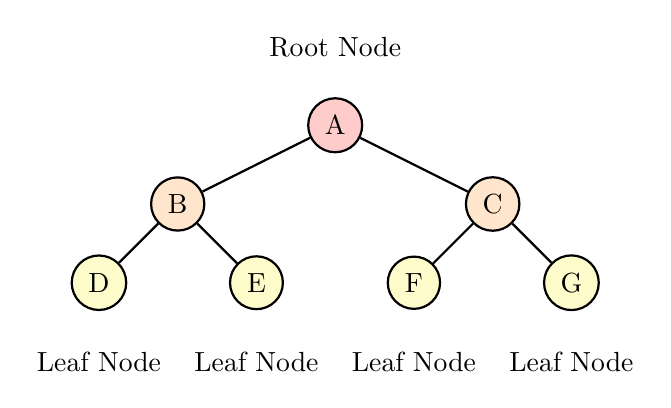
\begin{tikzpicture}
        \node[circle, draw, fill=red!20, thick] (A) at (0, 2) {A};
        \node[circle, draw, fill=orange!20, thick] (B) at (-2, 1) {B};
        \node[circle, draw, fill=orange!20, thick] (C) at (2, 1) {C};
        \node[circle, draw, fill=yellow!20, thick] (D) at (-3, 0) {D};
        \node[circle, draw, fill=yellow!20, thick] (E) at (-1, 0) {E};
        \node[circle, draw, fill=yellow!20, thick] (F) at (1, 0) {F};
        \node[circle, draw, fill=yellow!20, thick] (G) at (3, 0) {G};
        
        \node[above of=A] {\text{Root Node}};
        \node[below of=D] {\text{Leaf Node}};
        \node[below of=E] {\text{Leaf Node}};
        \node[below of=F] {\text{Leaf Node}};
        \node[below of=G] {\text{Leaf Node}};
        
        \draw[thick] (A) -- (B) -- (D);
        \draw[thick] (B) -- (E);
        \draw[thick] (A) -- (C) -- (F);
        \draw[thick] (C) -- (G);
    \end{tikzpicture}
    \caption{Example of a Tree}
\end{figure}

\section{Machine Learning Concepts}

A neural network is a function $f_\theta$ that maps the set of inputs $X$ to a set of outputs $Y$ with parameters $\theta$ (\cite{gurney2018introduction}).

An example of a neural network is an image classifier. An image classifier takes an input image $x \in X$, such as a handwritten digit, and maps it to a probability vector $f(x) \in Y$. This probability vector represents the likelihood of the image belonging to each possible class (\cite{kadam2020cnn}). 

\begin{figure}[htb]
    \centering
    \begin{equation*}
        f\left(\begin{gathered} 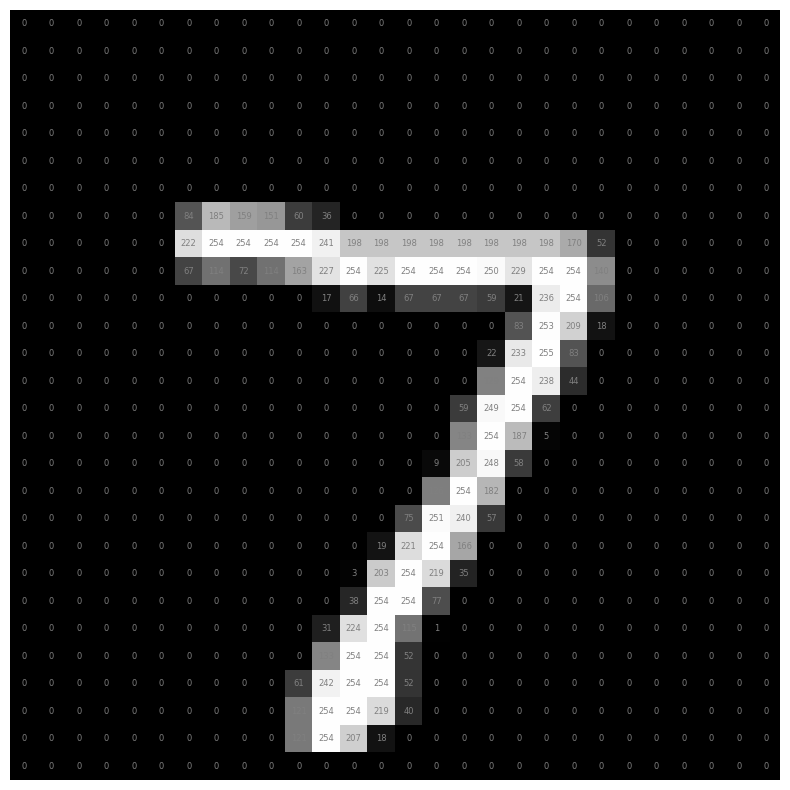
\includegraphics[width=0.28\linewidth]{images/neural_network_input_space.png} \end{gathered}\right) = \begin{bmatrix}
            \color{black!5} 0.0500 \\
            \color{black!5} 0.0500 \\
            \color{black!10} 0.1000 \\
            \color{black!20} 0.2000 \\
            \color{black!5} 0.0500 \\
            \color{black!1} 0.0100 \\
            \color{black!5} 0.0500 \\
            \color{black!47} 0.4700 \\
            \color{black!1} 0.0100 \\
            \color{black!1} 0.0100
        \end{bmatrix}
    \end{equation*}
    \caption{Example of a Neural Network Inference}
    \label{fig:nn-function}
\end{figure}

The image can be represented as a two-dimensional $28 \times 28$ matrix, where each element represents the luminosity of the pixel value. As shown in Figure \ref{fig:nn-function}, the function $f$ outputs a $1 \times 10$ probability vector where the zero-based index of the largest element represents what is the predicted value for the digit. In this case the highest value is at the $7^{th}$ position, then this means that the predicted value is the number $7$. 

% Here the neural network trains from a set $D$ composed of tuples with the first element being an image of a number represented as a $28\times 28$ matrix and the second one being the one-hot encoding representation of that number.

% One-hot encoding refers to the 

Neural networks are made up of one or more layers. Each layer accepts an input from previous layers and applies a differentiable function.

A linear layer applies the \verb|Linear| function defined by Equation \ref{eq:linear} to the input where $W$ is the weight matrix and $b$ is the bias vector. Both $W$ and $b$ are learnable parameters. The dimensions of the output of a linear layer depends on the dimensions of $W$ which can be configured. A linear layer is also called a dense layer.

\begin{equation}
    \verb|Linear|(x) = xW^T + b
    \label{eq:linear}
\end{equation}

A two-dimensional convolution layer applies the \verb|Conv2D| function defined by Equation \ref{eq:2dconvolution} where $x$ is the two-dimensional input represented as an $n \times m$ matrix, $b$ is the bias matrix, $(p_u, p_v)$ is the padding, and $W$ is the convolution matrix also known as the kernel with indexes from $-k_u$ to $k_u$ and $-k_v$ to $k_v$ for each dimension respectively. Both $W$ and $b$ are learnable parameters. The dimensions of the output of a two-dimensional convolution layer depends on the dimensions of $W$ which can be configured according to \cite{DBLP:journals/corr/OSheaN15}

\begin{equation}
    \verb|Conv2D|(x) = b + \sum_{u = p_u}^{n - p_u} \sum_{v = p_v}^{m - p_v} \sum_{\delta_u = -k_u}^{k_u} \sum_{\delta_v = -k_v}^{k_v} W(\delta_u, \delta_v) \cdot x(u + \delta_u, v + \delta_v)
    \label{eq:2dconvolution}
\end{equation}

A batch normalization layer applies the \verb|BatchNormalization| function defined by Equation \ref{eq:batch-normalization} to the input where $\gamma$ and $\beta$ are learnable parameters and $\epsilon$ is a small number typically equal to $1\times 10^{-5}$ (\cite{chollet2015keras}).

\begin{equation}
    \verb|BatchNormalization|(x) = \gamma \cdot \frac{x - \text{mean}{(x)}}{\sqrt{\text{variance}(x) + \epsilon}} + \beta
    \label{eq:batch-normalization}
\end{equation}

Activation layers applies a function to each element of the input. Non-linear activation layers introduces non-linearity to neural networks. Non-linear activation layers allows the neural network to model non-linear data (\cite{activation}).

A rectified linear unit (ReLU) layer is a non-linear activation layer that applies the \verb|ReLU| function defined by Equation \ref{eq:relu} to each of the element of its input (\cite{activation}). 

\begin{equation}
    \verb|ReLU|(x) =  \max\{0, x\}
    \label{eq:relu}
\end{equation}

A leaky ReLU layer is a generalization of the ReLU layer. A leaky ReLU is a non-linear activation layer that applies the \verb|LeakyReLU| function defined by Equation \ref{eq:leakyrelu} where $s$ is the slope of the values below $0$. When $s=0$, the leaky ReLU layer simplifies to the ReLU layer (\cite{activation}).

\begin{equation}
    \verb|LeakyReLU|(x) = \max{\{0, x\}} + s \cdot \min{\{0, x\}}
    \label{eq:leakyrelu}
\end{equation}

A flatten layer takes an input $x$ of any dimension and transforms it into a 1-dimensional array (\cite{chollet2015keras}).

% convolutional neural networks
% Similar to the paper by \cite{silver2017masteringchessshogiselfplay}, the model of \cite{Popic_Boskovic_Brest_2021} is a deep convolutional neural network (CNN). A CNN is a type of neural network that specializes on image classification due to their ability to recognize patterns in images. The rationale is that the model can learn to evaluate the positions of the pieces on the board and make appropriate moves accordingly because it is a CNN. 

% The main component of a CNN is a convolution layer. It

% As denoted in \cite{Popic_Boskovic_Brest_2021} the model contains convolution layers followed by normalization layers to stabilize the inputs and make the training faster and more stable. This layer is also called  called batch normalization as denoted by ``Normalization'' in Figure \ref{fig:popic-nn}.

\section{Training}

Training refers to the process of fitting the neural network to a set $D = \{ (x,\hat{y}) \mid x \in X, \hat{y} \in Y\}$ by minimizing a loss function $L(y, \hat{y})$ where $y = f(x)$ and $\hat{y}$ is the expected value of $f(x)$. The output of the neural network $y$ should converge to the expected value $\hat{y}$ within a certain loss $L$. 

A loss function is a function that calculates the divergence of the predicted value of the network $y$ by the true value $\hat{y}$ in the set $D$ (\cite{loss}). As opposed to layers, loss functions are not part of the neural network and are simply a means to evaluate the performance of the neural network.

Categorical cross-entropy is a loss function defined by Equation \ref{eq:cce}.

\begin{equation}
    \verb|CategoricalCrossEntropy| = -\sum_{i=1}^{n} \hat{y_i} \log y_i
    \label{eq:cce}
\end{equation}

Mean squared error is a loss function defined by Equation \ref{eq:mse}.

\begin{equation}
    \verb|MeanSquaredError| = \frac{1}{n}\sum_{i=1}^{n} (y_i - \hat{y_i})^{2}
    \label{eq:mse}
\end{equation}

L2 regularization is a loss function that penalizes high-value parameters in a neural network defined by Equation \ref{eq:l2} where $\lambda$ is the regularization constant.

\begin{equation}
    \verb|L2| = \lambda \sum_{i=1}^n\theta_i^2
    \label{eq:l2}
\end{equation}

Minimizing a loss function involves computing the gradients of each parameter of each layer of the neural network. Internally, modern machine learning libraries such as TensorFlow and PyTorch uses the backpropagation algorithm to achieve this (\cite{pytorch}).

The backpropagation algorithm first builds a directed acyclic graph of computation which is built during the forward pass and uses this structure to compute the gradient of each parameter. For instance, suppose $L = x + \sin(xy)$, to adjust the parameters $x$ and $y$ we need to compute $\dfrac{\partial L}{\partial x}$ and $\dfrac{\partial L}{\partial y}$.

\begin{figure}[htb]
    \centering
    \begin{subfigure}{0.4\textwidth}
        \centering
        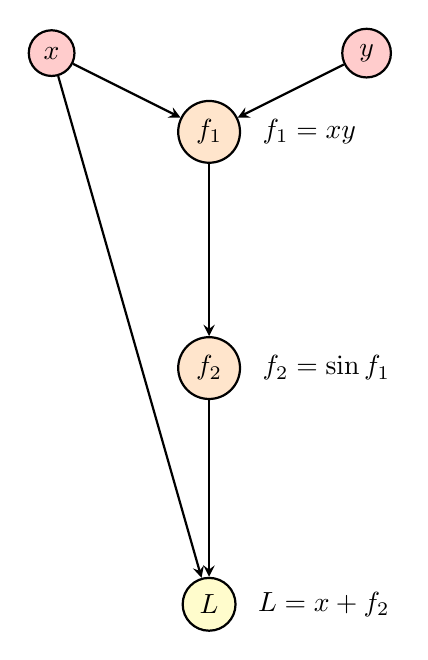
\begin{tikzpicture}
            \node[circle, draw, fill=red!20, thick] (x) at (1, 0) {$x$};
            \node[circle, draw, fill=red!20, thick] (y) at (5, 0) {$y$};
            \node[circle, draw, fill=orange!20, thick] (f1) at (3, -1) {$f_1$};
            \node[circle, draw, fill=orange!20, thick] (f2) at (3, -4) {$f_2$};
            \node[circle, draw, fill=yellow!20, thick] (L) at (3, -7) {$L$};
            
            \draw[thick, -stealth] (x) -- (f1);
            \draw[thick, -stealth] (y) -- (f1);
            \draw[thick, -stealth] (x) -- (L);
            \draw[thick, -stealth] (f1) -- (f2);
            \draw[thick, -stealth] (f2) -- (L);
            
            \node[right = 1.5mm of f1] (f1_label) {$f_1 = xy$};
            \node[right = 1.5mm of f2] (f2_label) {$f_2 = \sin f_1$};
            \node[right = 1.5mm of L] (f2_label) {$L= x + f_2$};
        \end{tikzpicture}
        \caption{Forward Pass}
        \label{fig:forward}
    \end{subfigure}
    \qquad
    \begin{subfigure}{0.4\textwidth}
        \centering
        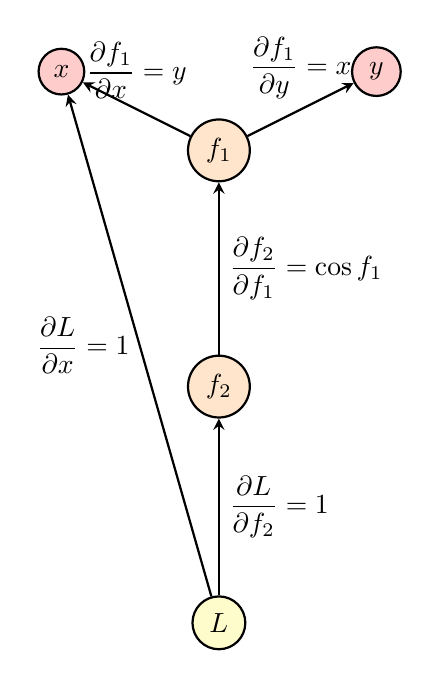
\begin{tikzpicture}
            \node[circle, draw, fill=red!20, thick] (x) at (1, 0) {$x$};
            \node[circle, draw, fill=red!20, thick] (y) at (5, 0) {$y$};
            \node[circle, draw, fill=orange!20, thick] (f1) at (3, -1) {$f_1$};
            \node[circle, draw, fill=orange!20, thick] (f2) at (3, -4) {$f_2$};
            \node[circle, draw, fill=yellow!20, thick] (L) at (3, -7) {$L$};
            
            \draw[thick, -stealth] (f1) -- node[above] {$\dfrac{\partial f_1}{\partial x} = y$} (x);
            \draw[thick, -stealth] (f1) -- node[above] {$\dfrac{\partial f_1}{\partial y} = x$} (y);
            \draw[thick, -stealth] (f2) -- node[right] {$\dfrac{\partial f_2}{\partial f_1} = \cos f_1$} (f1);
            \draw[thick, -stealth] (L) -- node[left] {$\dfrac{\partial L}{\partial x} = 1$} (x);
            \draw[thick, -stealth] (L) -- node[right] {$\dfrac{\partial L}{\partial f_2} = 1$} (f2);
        \end{tikzpicture}
        \caption{Backward Pass}
        \label{fig:backward}
    \end{subfigure}
    \caption{Anatomy of a Backpropagation}
    \label{fig:gradients}
\end{figure}

Backpropagation takes advantage of the fact that the partial derivative of a function with respect to a variable $x$, can be written in terms of the intermediate derivatives of each function, as shown in \ref{fig:backward}. In that example, 

\begin{equation}
    \frac{\partial L}{\partial x} = \frac{\partial L}{\partial x} + \frac{\partial L}{\partial f_2} \frac{\partial f_2}{\partial f_1} \frac{\partial f_1}{\partial x} = 1 + y\cos{xy}
\end{equation}

\begin{equation}
    \frac{\partial L}{\partial y} =\frac{\partial L}{\partial f_2} \frac{\partial f_2}{\partial f_1} \frac{\partial f_1}{\partial y} = x\cos{xy}
\end{equation}

An optimizer is an algorithm that adjusts the weights of each parameter to minimize the loss.

The Stochastic Gradient Descent (\verb|SGD|) with Momentum shown in Algorithm \ref{alg:sgdm} is an optimizer that replaces the actual gradient of the loss calculated from the entire set of data by an estimate calculated from a randomly selected subset of the data. The momentum keeps track of the update to the parameters at each iteration and determines the next update as a linear combination of the gradient and the previous update.

\begin{algorithm}[htb]
\caption{Stochastic Gradient Descent with Momentum}
\label{alg:sgdm}
\begin{algorithmic}
    \Require The learning rate $\eta$, loss function $\mathcal{L}$, momentum $\rho$, and learnable parameters $\theta$ of each layers of the neural network.
    \State $\delta \gets \nabla \mathcal{L}$
    \Function{SGD}{$\eta$, $\mathcal{L}$, $\rho$, $\theta$}
        \State $\delta  \gets \rho \delta - \eta\nabla\mathcal{L}$ 
        \State $\theta \gets \theta - \delta $
    \EndFunction{}
\end{algorithmic}
\end{algorithm}

% \begin{algorithm}[htb]
% \caption{Training Loop}
% \begin{algorithmic}
%     \State $e \gets 0 $
%     \While{$e \le \text{EPOCHS}$}
%         \State $(x, \hat{y}) \gets \text{Random}(D)$ 
%         \State $y \gets f_{\theta}(x)$
%         \State $L \gets \mathcal{L}(y, \hat{y})$
%         \State \Call{Backpropagate}{$f_{\theta}$, $L$}
%         \State \Call{Optimizer}{$f_{\theta}$}
%         \State $e \gets e + 1$
%     \EndWhile
% \end{algorithmic}
% \end{algorithm}

\section{Game Tree}

A sequential game is a game in which each player takes turns, that is, one player chooses their own action before the others choose theirs. Perfect information means that each player in the game knows the full state of the game and the history leading up to that state. An example of a sequential game is Chess and Checkers.

Sequential games can be represented using game trees that capture various game states as vertices of the tree and the actions applied on the current game state as edges. The root node of the tree corresponds to the initial game state, and each edge represents a decision made by a player, leading to a new game state. All the leaf nodes represents a terminal game state wherein the game may be a win, a lose, or a draw for the players.

\begin{figure}[htb]
    \centering
    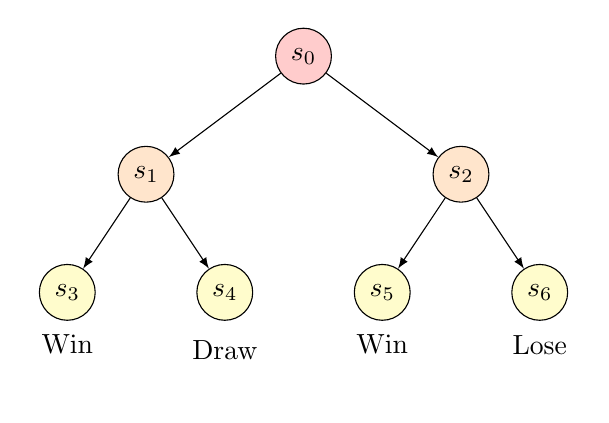
\begin{tikzpicture}[
      level 1/.style={sibling distance=40mm},
      level 2/.style={sibling distance=20mm},
      edge from parent/.style={draw,-latex},
      every node/.style={circle,draw,minimum size=7mm},
      label/.style={below=4pt, draw=none, fill=none}
      ]
      \node[fill=red!20] {$s_0$}
        child {node[fill=orange!20] {$s_1$}
          child {node[fill=yellow!20] {$s_3$} node[label] {Win}}
          child {node[fill=yellow!20] {$s_4$} node[label] {Draw}}
        }
        child {node[fill=orange!20] {$s_2$}
          child {node[fill=yellow!20] {$s_5$} node[label] {Win}}
          child {node[fill=yellow!20] {$s_6$} node[label] {Lose}}
        };
    \end{tikzpicture}
    \caption{Game Tree}
    \label{fig:game-tree}
\end{figure}

For simple games such as tic-tac-toe, all game states can be exhaustively analyzed by a computer and make it so that it produces the theoretically optimal winning move given a state. However, this is infeasible and computationally expensive for games such as Go and Chess. For instance, according to  \cite{jontromp}, the game of Go has been calculated to have approximately $2.1 \times 10^{170}$ possible moves, which is larger than the number of atoms in the universe. That means, it is  impossible to be approached this way. % cite

One approach to mitigate this is to approximate the optimal move by walking through only a finite nodes of the tree. Such an approach is employed by the AlphaZero framework and was used to beat professionals on games such as chess, go, and shogi.

\section{The AlphaZero Framework}

The AlphaZero framework is a general reinforcement learning algorithm by \cite{silver2017masteringchessshogiselfplay} that has shown success in conquering sequential games such as chess, go, and shogi. This framework can be applied to any sequential games with perfect information. This framework has three major components: the Monte-Carlo Tree Search Algorithm, a deep neural network, and reinforcement learning through self-play.

According to \cite{silver2017masteringchessshogiselfplay}, AlphaZero uses a general-purpose Monte-Carlo tree search (MCTS) algorithm. Each search consists of a series of simulated games of self-play that traverse a game tree from root $s_{root}$ to leaf. Each simulation proceeds by selecting in each state $s$ a move $a$ with low visit count $N(s, a)$, high move probability $P(s,a)$ and high value $Q(s, a)$ according to the current neural network $f_\theta$. The search returns a vector $\pi$ representing a probability distribution over moves, either proportionally or greedily with respect to the visit counts at the root state.

Each state-action pair $(s,a)$ stores a set of statistics, $\{N(s, a), W(s, a), Q(s, a), P(s, a)\}$, where $N(s, a)$ is the visit count, $W(s, a)$ is the total action-value, $Q(s, a)$ is the mean action-value, and $P(s, a)$ is the prior probability of selecting $a$ in $s$, as shown in Figure \ref{fig:game-tree-with-stats}.

\begin{figure}[htb]
    \centering
    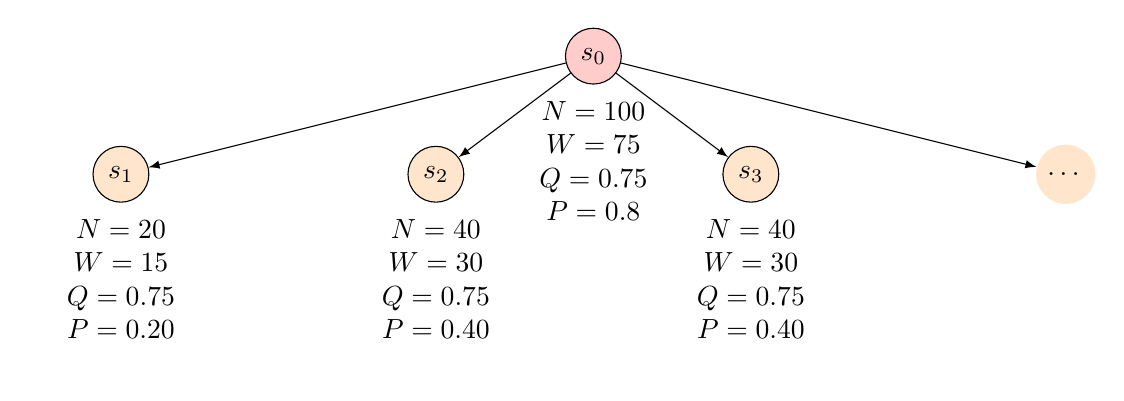
\begin{tikzpicture}[
      level 1/.style={sibling distance=40mm},
      level 2/.style={sibling distance=20mm},
      edge from parent/.style={draw,-latex},
      every node/.style={circle,draw,minimum size=7mm},
      label/.style={below=4pt, draw=none, fill=none, align=center}
      ]
      \node[label] {$N = 100$\\$W = 75$\\$Q = 0.75$\\$P = 0.8$} node[fill=red!20] {$s_0$}
        child {node[fill=orange!20] {$s_1$} node[label] {$N = 20$\\$W = 15$\\$Q = 0.75$\\$P = 0.20$}}
        child {node[fill=orange!20] {$s_2$} node[label] {$N = 40$\\$W = 30$\\$Q = 0.75$\\$P = 0.40$}}
        child {node[fill=orange!20] {$s_3$} node[label] {$N = 40$\\$W = 30$\\$Q = 0.75$\\$P = 0.40$}}
        child {node[fill=orange!20, draw=none] {$\dots$}};
    \end{tikzpicture}
    \caption{State-Action Pairs Storing a Set of Statistics}
    \label{fig:game-tree-with-stats}
\end{figure}

Each simulation begins at the root node of the search tree, $s_0$, and finishes when the simulation reaches a leaf node $s_L$ at time-step $L$, as shown in Figure \ref{fig:root-to-leaf}.

\begin{figure}[htb]
    \centering
    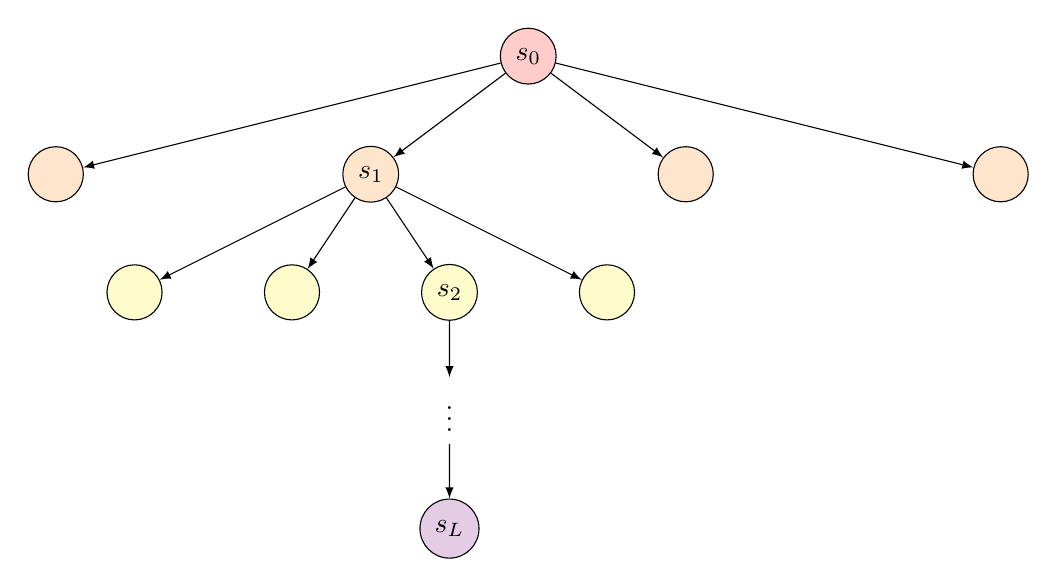
\begin{tikzpicture}[
      level 1/.style={sibling distance=40mm},
      level 2/.style={sibling distance=20mm},
      edge from parent/.style={draw,-latex},
      every node/.style={circle,draw,minimum size=7mm},
      label/.style={below=4pt, draw=none, fill=none, align=center}
      ]
      \node[fill=red!20] {$s_0$}
        child {node[fill=orange!20] {}}
        child {node[fill=orange!20] {$s_1$}
            child {node[fill=yellow!20] {}}
            child {node[fill=yellow!20] {}}
            child {node[fill=yellow!20] {$s_2$}
                child {node[draw=none] {$\vdots$}
                    child {node[fill=violet!20] {$s_L$}}}}
            child {node[fill=yellow!20] {}}}
        child {node[fill=orange!20] {}}
        child {node[fill=orange!20] {}};
    \end{tikzpicture}
    \caption{Simulation of MCTS on the Search Tree}
    \label{fig:root-to-leaf}
\end{figure}

At each of these time-steps, $t < L$, an action is selected $a_t = \operatorname{arg} \operatorname{max}_a \big(Q(s_t, a_t) + U(s_t, a_t)\big)$, using a variant of the Predictor + Upper-Confidence Bound Applied to Trees (PUCT) algorithm, $U(s, a) =  C(s) P(s, a) \sqrt{N(s)} / (1 + N(s, a))$, where $N(s)$ is the parent visit count and $C(s)$ is the exploration rate, which grows slowly with search time, $C(s) = \log\left((1 + N(s) + c_{base}) / c_{init}\right) + c_{init}$, but is essentially constant during the fast training games. The leaf node $s_L$ is added to a queue for neural network evaluation, $(\mathbf{p}, v) = f_\theta(s)$. The leaf node is expanded and each state-action pair $(s_L, a)$ is initialized to $\{N(s_L, a) = 0, W(s_L, a) = 0, Q(s_L, a) = 0, P(s_L, a) = p_a\}$. The visit counts and values are then updated in a backward pass through each step $t \leq L$, $N(s_t, a_t) = N(s_t, a_t) + 1$, $W(s_t, a_t) = W(s_t, a_t) + v$, $Q(s_t, a_t) = W(s_t,a_t) / N(s_t,a_t)$.

% During each search, a root node is The MCTS used in AlphaZero has four phases: selection, expansion, simulation, and backpropagation. The selection phase traverses the tree and make use of the Predictor + Upper-Confidence Bound Applied to Trees (PUCT) formula introduced by AlphaGo for the selection of nodes, balancing exploitation of nodes with higher estimated value with the exploration of least visited nodes. It continues down the tree until reaching a node that has not been fully expanded or explored. It does so by traversing through the nodes which has the largest PUCT score.

% $Q(s, a)$ is the average value of leaf states from the simulations that selected $a$ from $s$. 

% \begin{equation}\label{eq:q}
%     Q(s, a) = \frac{W(s, a)}{N(s, a)}
% \end{equation}
% \begin{equation}\label{eq:u}
%     U(s, a) = C(s) P(s, a) \sqrt{N(s)} \cdot \frac{1}{1 + N(s, a)}
% \end{equation}
% \begin{equation}\label{eq:cs}
%     C(s) = \log\left(\frac{1 + N(s) + c_{base}}{c_{init}}\right) + c_{init}
% \end{equation}

% The PUCT formula is defined by Equation \ref{eq:puct} where $C(s)$ is the exploration rate that grows slowly with the number of iterations $i$, $c_{base}$ and $c_{init}$ are constants chosen arbitrarily by AlphaZero, $v_i$ is the evaluated value of node $s$, $n_i$ is total number of visits of node $s$, and $N_i$ is the total number of visits of the parent node of $s$.

% \begin{equation}\label{eq:puct}
%     PUCT(s) = Q(s, a) + U(s, a)
% \end{equation}

% Once a node is selected, if it is not a terminal node, the algorithm generates one or more child nodes corresponding to possible moves from that state. This expands the tree by adding new game states for exploration.

% From the newly added node, the algorithm runs a random simulation of the game by selecting moves randomly until it reaches a terminal state. The outcome of the simulation (win, loss, draw, etc.) is recorded.

% The result of the simulation is then propagated back up the tree to update the statistics of the nodes along the path taken during selection. This step helps the algorithm adjust its understanding of which moves are more likely to result in favorable outcomes.

% Putting all these together we get the MCTS

% \begin{algorithm}[htb]
% \begin{algorithmic}[1]
%     \Function{MCTS}{$root, N_{max}$}
%         \State $N \gets 0$
%         \Repeat 
%             \State $leaf \gets \Call{Traverse}{root}$
%             \State $value \gets \Call{Simulate}{leaf}$
%             \State $\Call{Backpropagate}{leaf, value}$
%             \State $N \gets N + 1$
%         \Until{$N = N_{max}$}
%         \State \Return the child of $root$ with the highest number of visits
%     \EndFunction
% \end{algorithmic}
% \end{algorithm}

% \begin{algorithm}[htb]
% \begin{algorithmic}[1]
%     \Function{Traverse}{$node$}
%         \While{$node$ is a fully expanded node}
%             \State $node$ is assigned the child node of $node$ with the maximum PUCT score.
%         \EndWhile
%         \State \Return $\Call{UnvisitedChild}{node}$ or $node$
%     \EndFunction
% \end{algorithmic}
% \end{algorithm}

% \begin{algorithm}[htb]
% \begin{algorithmic}[1]
%     \Function{Simulate}{$node$}
%         \While{$node$ is a non-terminal node}
%             \State $node$ is assigned to a random children of $node$
%         \EndWhile
%         \State \Return $\Call{GetOutcome}{node}$
%     \EndFunction
% \end{algorithmic}
% \end{algorithm}

% \begin{algorithm}[htb]
% \begin{algorithmic}[l]
%     \Function{Backpropagate}{$node$, $value$}
%             \If{$node$ has no parent}
%                 \State \Return 
%             \EndIf

%             \State $\Call{UpdateParameters}{node, value}$
%             \State $\Call{Backpropagate}{\Call{GetParent}{node}, value}$
%     \EndFunction
% \end{algorithmic}
% \end{algorithm}

According to \cite{silver2017masteringchessshogiselfplay}, AlphaZero utilizes a deep neural network $(\mathbf{p}, v) = f_\theta(s)$ with parameters $\theta$. This neural network takes the board position $s$ as an input and outputs a vector of move probabilities $\mathbf{p}$ with components $p_a = Pr(a|s)$ for each action $a$, and a scalar value $v$ estimating the expected outcome $z$ from position $s$, $v \approx \mathbb{E}[z|s]$. AlphaZero learns these move probabilities and value estimates entirely from self-play; these are then used to guide its search.

According to \cite{silver2017masteringchessshogiselfplay}, the parameters $\theta$ of the deep neural network in AlphaZero are trained by self-play reinforcement learning, starting from randomly initialized parameters $\theta$. Games are played by selecting moves for both players by MCTS, $a_t \sim \mathbf{\pi}_t$. At the end of the game, the terminal position $s_T$ is scored according to the rules of the game to compute the game outcome $z$: $-1$ for a loss, $0$ for a draw, and $+1$ for a win. The neural network parameters $\theta$ are updated so as to minimize the error between the predicted outcome $v_t$ and the game outcome $z$, and to maximize the similarity of the policy vector $\mathbf{p}_t$ to the search probabilities $\pi_t$. Specifically, the parameters $\theta$ are adjusted by gradient descent on a loss function $l$ than sums over mean-squared error and cross-entropy losses respectively,

\begin{equation}\label{eq:loss}
    (\mathbf{p}, v) = f_\theta(s), \qquad l = (z - v)^2 - \pi^\top \log \mathbf{p} + c\lVert\theta\rVert^2
\end{equation}

where $c$ is a parameter controlling the level of $L_2$ weight regularisation. The updated parameters are used in subsequent games of self-play.

\section{Deep Learning and the Game of Checkers}

% paraphrase
Based on a study conducted by \cite{Popic_Boskovic_Brest_2021}, they were able to train a deep convolutional neural network based on the AlphaZero framework that was able to learn how to play the game of German checkers defined in their paper through self-play with each new version representing a better player. \cite{Popic_Boskovic_Brest_2021} focused on the rules of German checkers in which the game is played on an $8 \times 8$ board with interchanging black and white squares. There are 12 white and 12 black playing figures that are coin like shaped. Each player has their figures arranged on black squares in first 3 rows closest to them as shown in Figure \ref{fig:checkers-start}. 

\begin{figure}[htb]
    \centering
    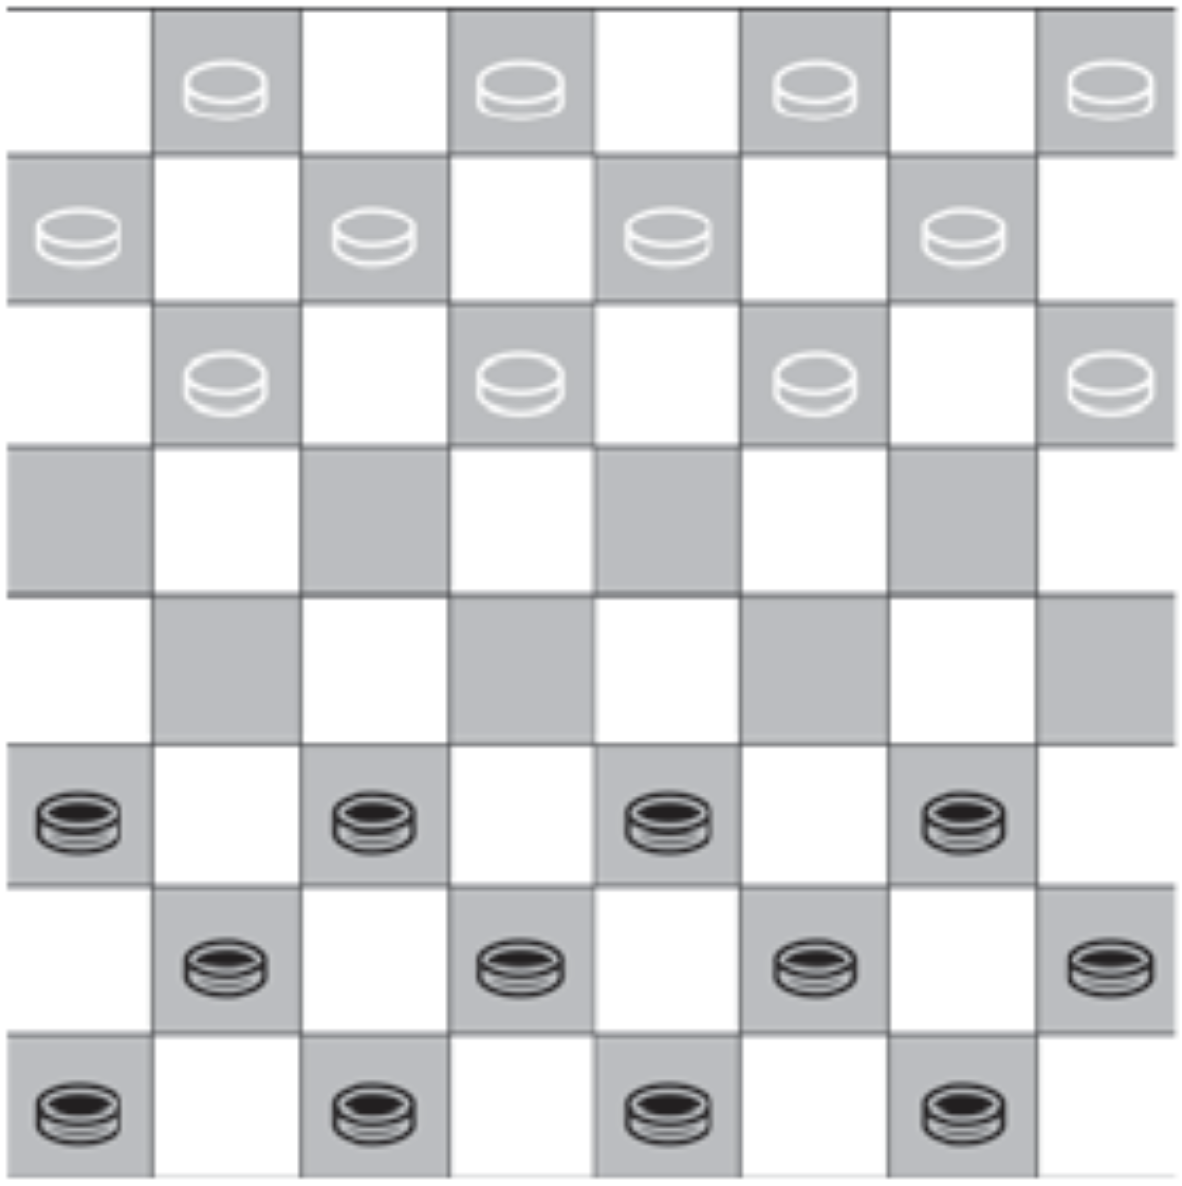
\includegraphics[width=0.3\textwidth]{images/checkers.png}
    \caption{Starting State of the Board in German Checkers used in \cite{Popic_Boskovic_Brest_2021}}
    \label{fig:checkers-start}
\end{figure}

A game of German checkers is always started by the player with black figures and is continued by the opponent. Regular game figures can only move diagonally on black squares towards the opponent’s side one square at a time. If there is an opponent’s figure in the path of the move and a square behind that figure is vacant, the player must capture the opponent’s figure by jumping over it and removing it from the playing board. If multiple such successive captures exist, the player must perform them all in one move.

If the player reaches the opponent’s side of the board, the player’s figure is knighted and gains the ability to move diagonally forward and backward for any number of squares at a time. A game is won if the opponent has no figures left on the board or is out of possible legal moves. The game ends in a draw if no pieces have been captured in the last 40 moves.

Two player agents with their own game tree and neural network were used in \cite{Popic_Boskovic_Brest_2021}. Each agent gets a list of possible legal moves it can make on its turn from the game environment. It also has a whole overview of the game state at any given time where it has full knowledge where the opponent has its figures and what type of figures they are.

\begin{table}[htb]
    \centering
    \begin{tabular}{lll}
        \hline
        Parameter & Value & Description \\ \hline
        \verb!EPISODES! & 50 & number of self-play games for data creation \\
        \verb!MCTS_SIMS! & 70 & number of MCTS iterations \\
        \verb!TURNS_UNTIL_TAU0! & 25 & number of moves after the game is played deterministically \\
        \verb!BATCH_SIZE! & 256 & batch size used for learning \\
        \verb!LEARNING_RATE! & 0.1 & learning rate \\
        \verb!MOMENTUM! & 0.9 & learning momentum \\
        \verb!EVAL_EPISODES! & 20 & number of games played in validation phase \\
        \verb!SCORING_THRESHOLD! & 1.3 & scoring factor in validation phase \\ \hline
    \end{tabular}
    \caption{Algorithm Parameters in \cite{Popic_Boskovic_Brest_2021}}
    \label{tab:algo-params}
\end{table}

During every turn, the agent uses the MCTS algorithm with parameters shown in Table \ref{tab:algo-params} to select the best move from the list of possible legal moves. Random move selection were used for the first \verb!TURNS_UNTIL_TAU0! game moves to further explore new and different game scenarios during the learning phase of the neural network.

Before the agent selects a move from the current game state $s$, the MCTS algorithm runs for \verb!MCTS_SIMS! iterations. Each node of the game tree represents a certain move $a$ and contains the number of node visits $N(s, a)$, its value $Q(s, a)$ and probability of selecting that move $P(s, a)$ received from the neural network. The current node value $Q(s, a)$ represents the mean value of its branch and is calculated from its leaf value $V(s^i_L)$ returned by the neural network, current node visit counter $N(s, a)$, and $l(s, a, i)$ which represents if the leaf $i$ was visited from the current node as shown in Equation \ref{eq:qsa}.

\begin{equation} \label{eq:qsa}
    Q(s, a) = \frac{1}{N(s,a)} \sum_i l(s, a, i) V(s^i_L) 
\end{equation}

The algorithm starts from the root node and continuously select moves $a$ that maximize the score $S(s, a) = Q(s, a) + u(s, a)$ where $u(s, a) \propto \frac{P(s,a)}{1+N(s,a)}$. $u(s, a)$ is used to improve the exploration of moves that have not been selected often and exploit moves that already have a sufficiently high prior probability $P(s, a)$ of being selected. During each node visit, the node's values are updated and the node's position are evaluated with the neural network if a leaf was reached. A move from the children of the root node which has the highest value $Q(s, a)$ is selected after \verb!MCTS_SIMS! iterations of tree traversal.

\begin{figure}[htb]
    \centering
    \begin{subfigure}{0.4\textwidth}
        \centering
        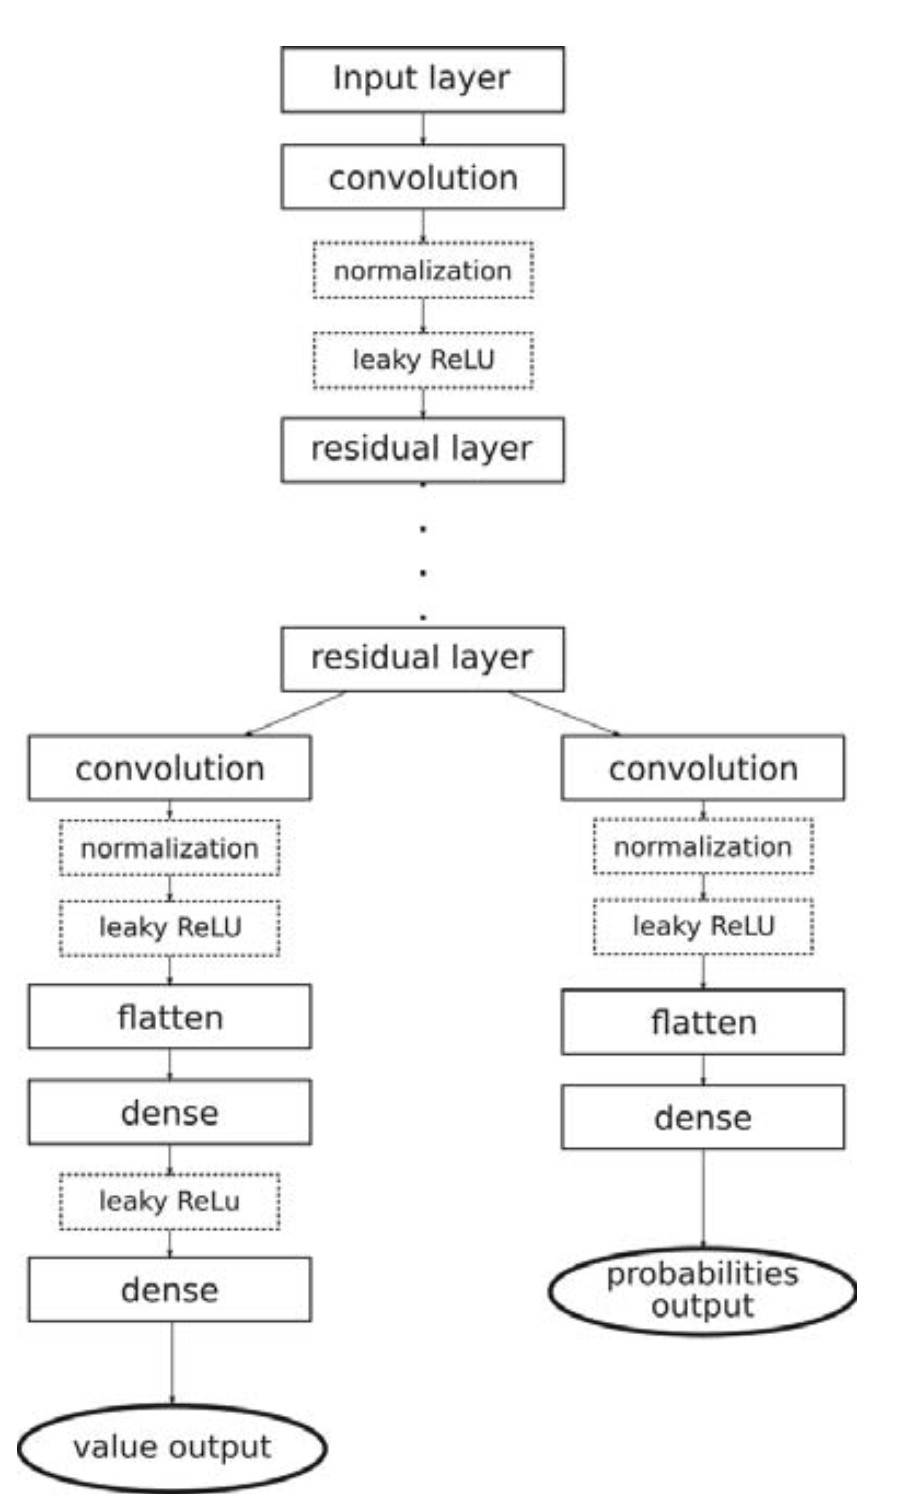
\includegraphics[scale=0.25]{images/checkers_nn.png}
        \caption{Deep Neural Network Architecture}
        \label{fig:dnn}
    \end{subfigure}
    \qquad
    \begin{subfigure}{0.4\textwidth}
        \centering
        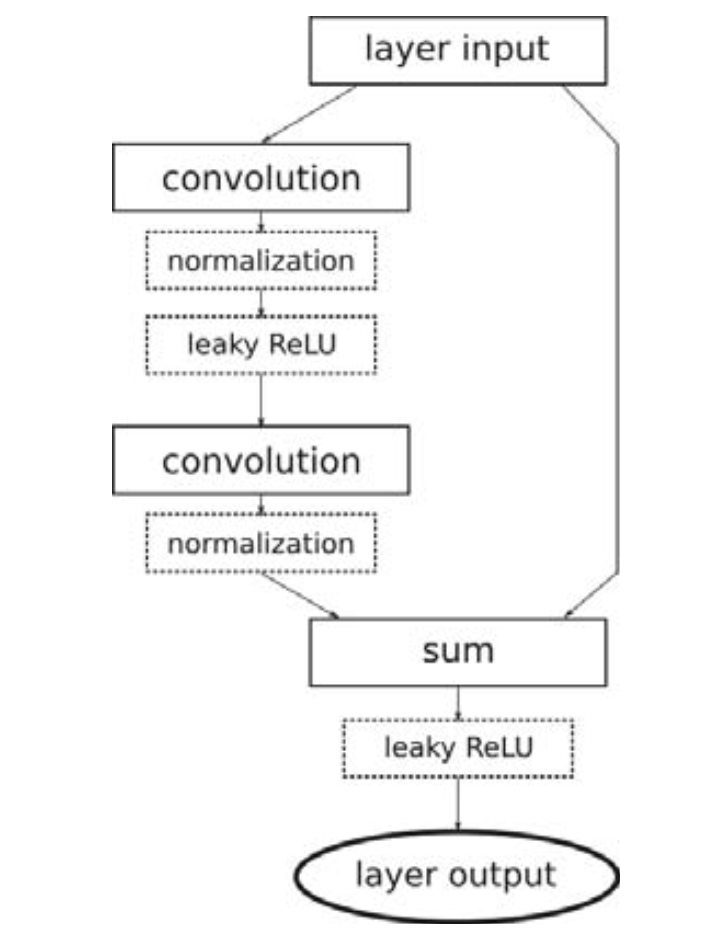
\includegraphics[scale=0.25]{images/residual_layer.png}
        \caption{Anatomy of a Residual Layer}
        \label{fig:residual}
    \end{subfigure}
    \caption{Overview of the Deep Neural Architecture used in \cite{Popic_Boskovic_Brest_2021}}
    \label{fig:popic-nn}
\end{figure}


The structure of the neural network used in \cite{Popic_Boskovic_Brest_2021} follows the architecture used in \cite{silver2017masteringchessshogiselfplay}. The input in the neural network is a matrix of size $2 \times 8 \times 8$ which describes the current game state, the first and second layer for the pieces of the first and second player, respectively. The numbers $-1$, $-2$, $1$, and $2$ are used to represent two different pieces for each player: normal and knighted pieces for white and black, respectively. After the input layer, there is a convolution layer with 75 kernels of size $4 \times 4$, followed by 5 residual layers. The overall structure is shown in Figure \ref{fig:dnn}.

Each residual layer consists of 2 convolutions with 75 kernels of size $4 \times 4$ followed by addition of this convolutions and layer input. Residual layer is represented in Figure \ref{fig:residual}. After every convolutional layer, the paper utilized batch normalization to speed up the learning and mitigate overfitting.

The neural network has 2 outputs. The first output is the result of a convolution layer, flattening layer and two dense layers which reduce the dimension to one value. This value represents value $V$ of the current board state. 
The second output is achieved by a convolution layer, that is again followed by flattening, and a dense layer which reduces the dimension to a vector of size 64. This represents the probability for each position. This output probability vector is of size 64 corresponding to the unraveled $8 \times 8$ board. This vector represents the probability distribution over possible new board states, not specific move pairs.

The neural network utilizes leaky ReLU activation function and stochastic gradient descend with momentum to adjust network weights and kernels.
x
The work in \cite{Popic_Boskovic_Brest_2021} consists of learning through self-play between two versions of the neural network. The general flow chart can be seen in Figure \ref{fig:self-play}. Data needed for learning is generated by playing a number of games provided by the \verb!EPISODES! parameter between an agent using the current neural network and an agent using the best neural network. Both neural networks are the same in the first iteration. During the data creation phase, every game is started by an agent that moves randomly, thus eliminating any advantage a starting player would have. After each game, the game states and normalized visit counts are saved from the MCTS algorithm.

\begin{figure}[htb]
    \centering
    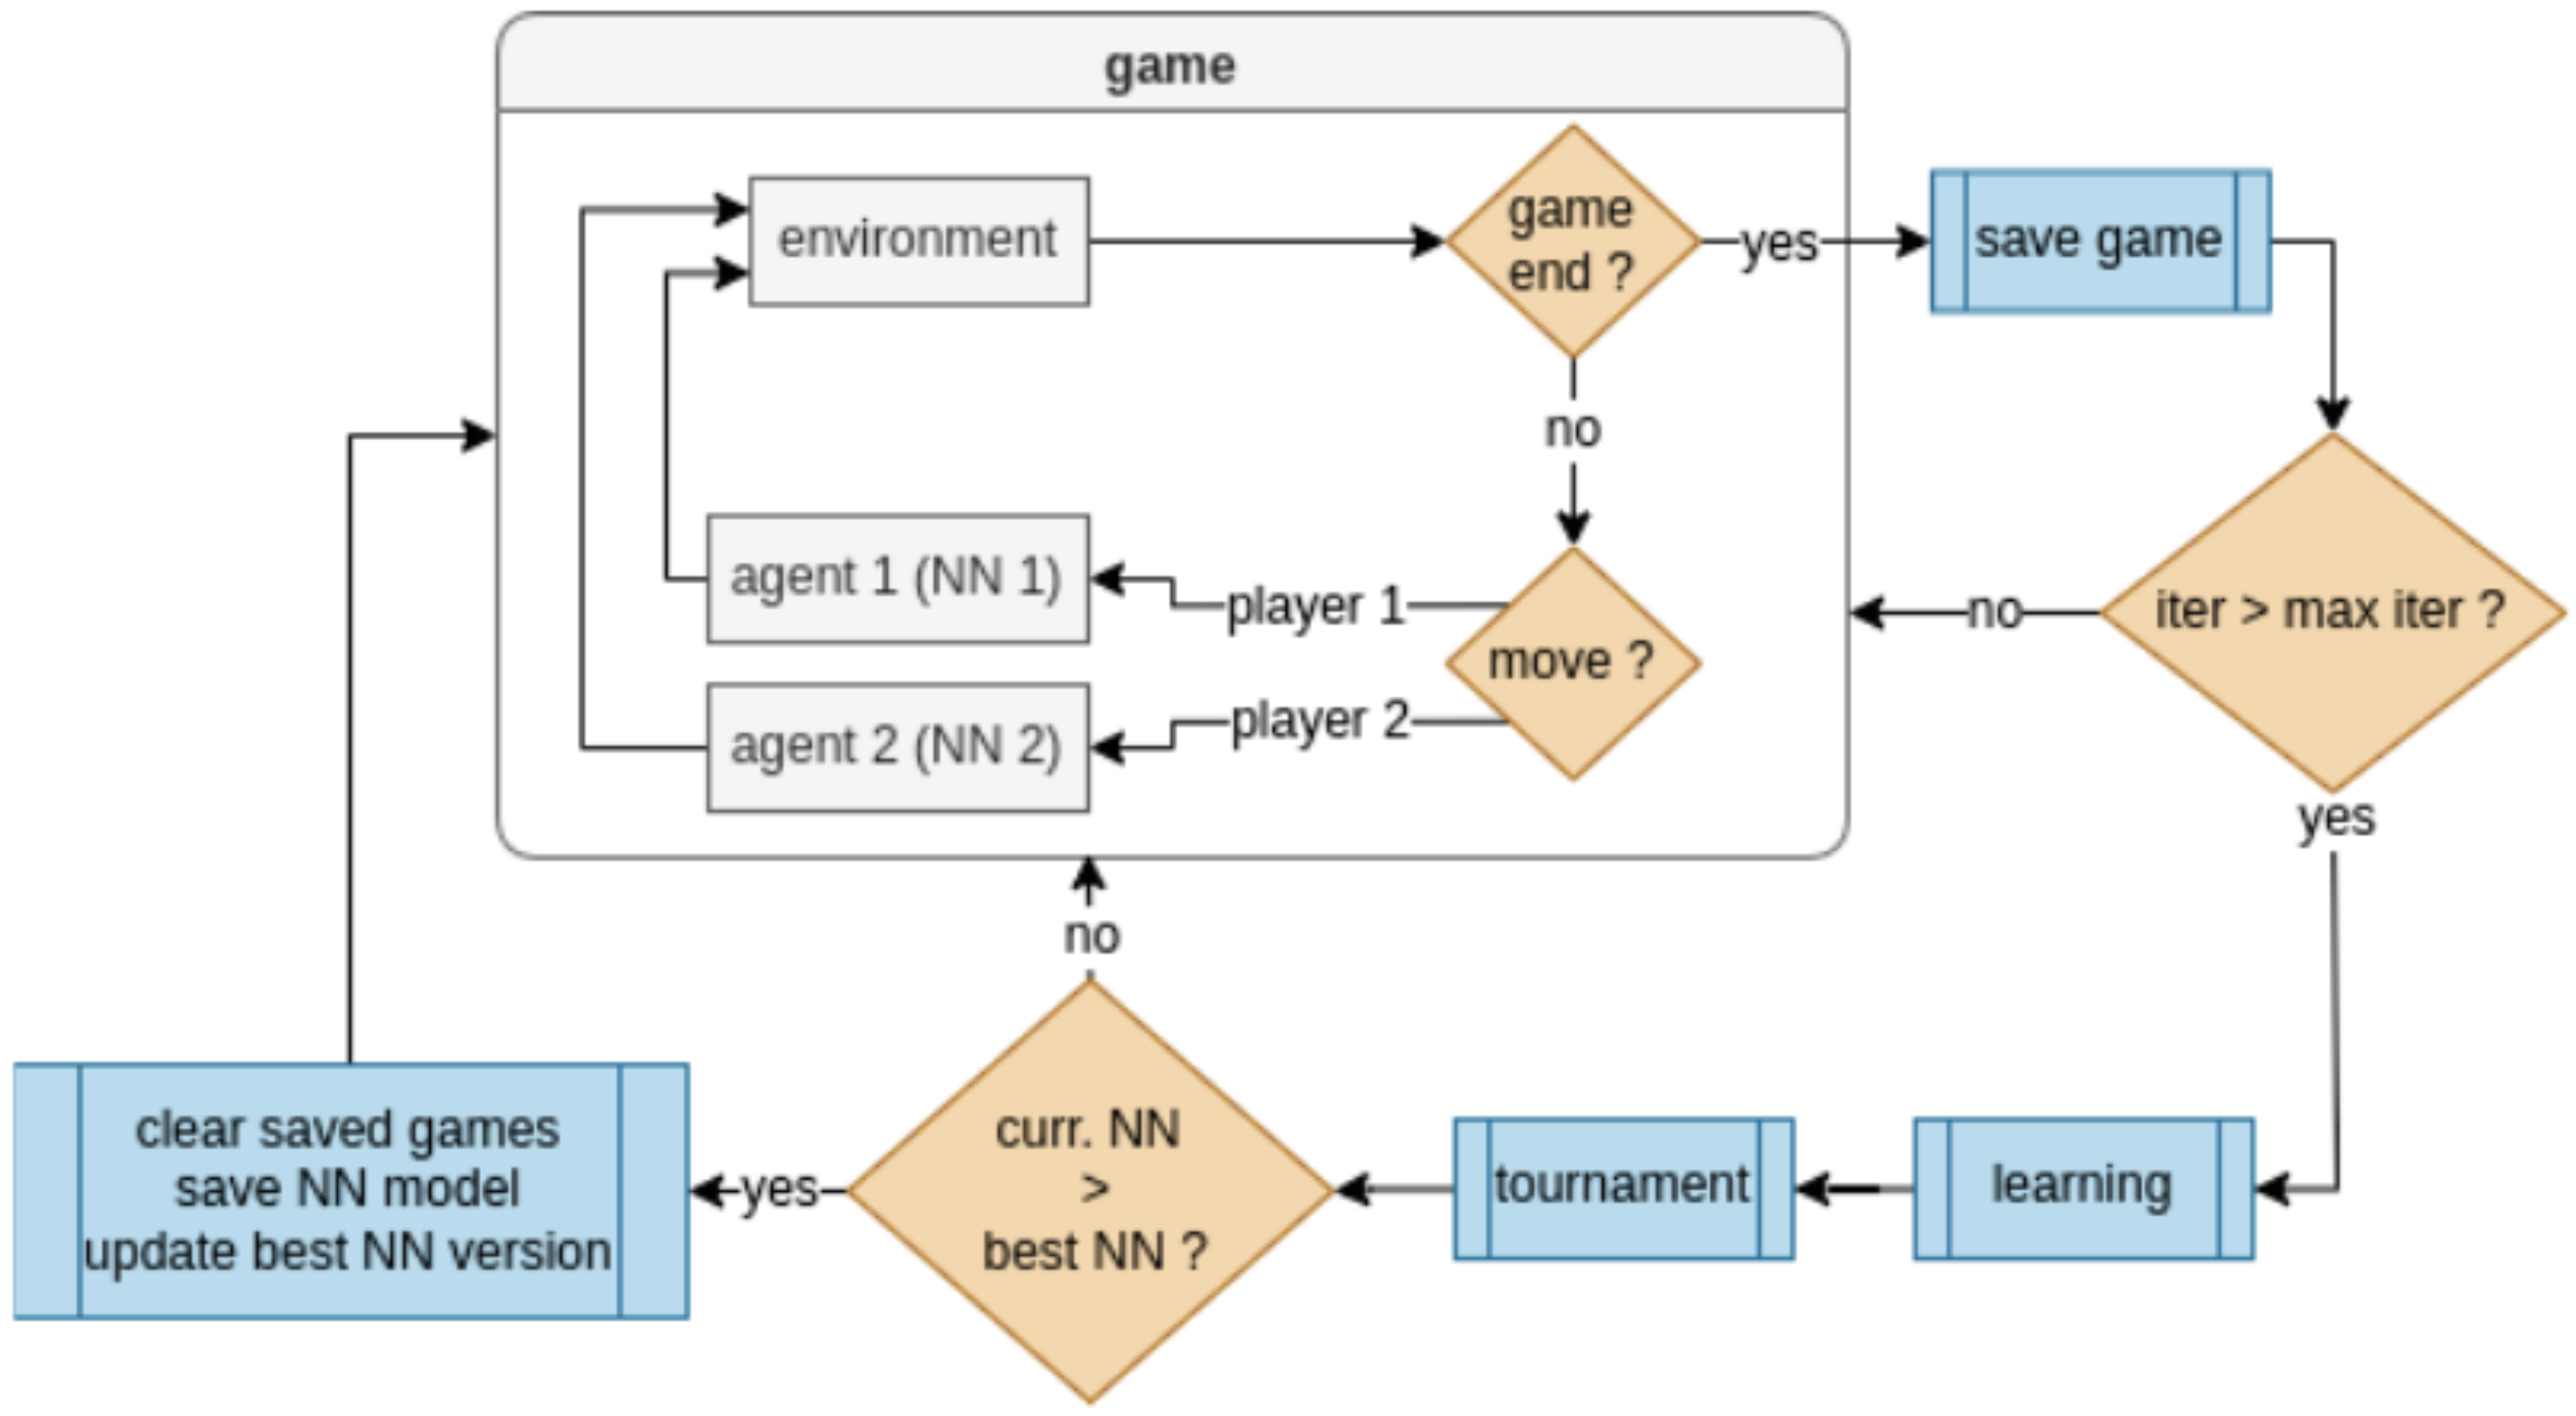
\includegraphics[width=0.7\linewidth]{images/self-play.png}
    \caption{General Flow Chart in \cite{Popic_Boskovic_Brest_2021}}
    \label{fig:self-play}
\end{figure}

After the data creation phase, the learning phase is initialized. During this phase, the generated data is used to train the current neural network with reinforcement learning combined with input batches.

After the learning phase, a tournament is started between the agent using the newly trained neural network and the one using the currently best neural network. During the tournament phase, \verb!EVAL_EPISODES! games are played. Each agent is scored according to the chess scoring where 3 points is given for a win, 1 point for a draw and 0 points for a loss. The newly trained neural network is deemed the current best if the agent using the newly trained neural network has obtained more points than the agent using the currently best neural network by a ratio defined by the \verb!SCORING_THRESHOLD! parameter after the completion of the tournament phase and the whole process is repeated again.

\cite{Popic_Boskovic_Brest_2021} ran the algorithm as described with parameters seen in Table \ref{tab:algo-params}. Instead of discarding the older neural network model when a better one was found, \cite{Popic_Boskovic_Brest_2021} saved that version for later use. After approximately 2 weeks of runtime, \cite{Popic_Boskovic_Brest_2021} were able to obtain 9 different versions of the neural network model, each being better than the previous one. \cite{Popic_Boskovic_Brest_2021} ran fifty games between an agent using the ninth version of the neural network model marked as the best and agents using every other versions of the neural network. Every game was scored according to the chess scoring. Number of wins (W), draws (D), and losses(L) of the ninth version of the neural network versus other versions as well as the final score (S) can be seen in Table \ref{tab:v9_summary}.

\begin{table}[htb]
    \centering
    \begin{tabular}{c|cccccccccc}
        & v0 & v1 & v2 & v3 & v4 & v5 & v6 & v7 & v8 & v9 \\ \hline
        W & 32 & 27 & 26 & 33 & 29 & 26 & 18 & 11 & 14 & 17 \\
        D & 13 & 18 & 19 & 10 & 17 & 13 & 16 & 20 & 14 & 16 \\
        L & 5 & 5 & 5 & 7 & 4 & 11 & 16 & 19 & 22 & 17 \\ \hline
        S & 109 & 99 & 97 & 109 & 104 & 91 & 70 & 53 & 56 & 67
    \end{tabular}
    \caption{Games of the Agent using the Ninth Version of the Neural Network Against All Other Versions of the Neural Network in \cite{Popic_Boskovic_Brest_2021}}
    \label{tab:v9_summary}
\end{table}

The final scores against lower and worse versions of the neural network are generally higher than those against higher and better versions. The number of wins generally decreases and the number of losses generally increases. The ninth version of the neural network obtained the same number of wins and losses when playing against itself, as shown in the ninth column of Table \ref{tab:v9_summary}, which is on par with the idea that two equivalent players will have the same chances of winning and losing.

The paper by \cite{Popic_Boskovic_Brest_2021} managed to demonstrate the ability of an AlphaZero-based approach to learning the game of Checkers when given only the game rules. The approach is only given a set of game rules. The data needed to train newer models of neural network are generated by self-play. Nine different versions of the neural network were obtained after two weeks of runtime, each better than the previous one. Some discrepancies are seen with regards to the score achieved by the first few versions, which is most likely due to noise and could be addressed by optimizing the \verb|EPISODES|, \verb|EVAL_EPISODES|, and \verb|SCORING_THRESHOLD| parameters according to \cite{Popic_Boskovic_Brest_2021}.


\section{The Game of Damath}

Damath comes from the Filipino checkers called ``dama'' and mathematics. According to \cite{MathleteSociety2024}, Damath was created by Jesus Huenda, a teacher in the province of Sorsogon, Philippines who was inspired by his student named Emilio Hina Jr. for his submission of an investigatory project called ``Dama de Numero'' in 1975. Huenda developed and refined the game, first introducing it to his students. The popularity of the game grew rapidly, leading to the first Damath tournament being held in Sorsogon in 1980.  The innovative approach of Huenda to teaching mathematics earned him a gold medallion from the late President Ferdinand Marcos in 1981. The popularity of Damath reached its peak in the 1990s, with the game being featured at numerous mathematics education conventions around the world, including conferences in Australia, Thailand, Malaysia, and Korea. In 2011, Damath was introduced to the United States by Reynaldo L. Duran, an international Filipino educator, at the National Council of Teachers of Mathematics (NCTM) conference in New Mexico.

Damath is very similar to the game of Checkers, except that the checkerboard has the basic mathematical operations (addition, subtraction, multiplication and division) on each playable tiles which dictates the operation that will be used when a piece of a player captures the piece of an opponent. It has numbers labeled 0-7 on its sides to determine the coordinates of the piece. Each piece of the player has corresponding values depending on what type of damath is being played. Both board and damath pieces are mostly made of thick cardboard or illustration board.

\begin{figure}[htb]
     \centering
     \includegraphics[width=0.5\linewidth]{images/initial_state.png}
     \caption{Initial State of Damath}
     \label{fig:initial_state}
\end{figure}
 
If there is an opponent's figure in the path of the move and the square behind that figure is vacant, the player must capture the opponent's figure by jumping over it and removing it from the playing board. The capturing figure must perform a calculation based on the mathematical operator where the capturing figure lands. If multiple such successive captures exist, the player must perform them all in one move. The result of the calculation is added to the score of the player who captured the piece.

If the player reaches opponent’s side of the board, the player's figure turns into a dama and hence has the ability to move diagonally forward and backward. Game is won if the opponent has no figures left on the board or is out of possible legal moves. The game ends in a draw if no pieces have been captured in the last 40 moves.
 

\section{Existing AI Models for Damath}

Although AI in Damath is less explored than in other board games, a few existing models attempt to simulate intelligent play within the rules of the game. These models are often based on rule-based algorithms or basic decision trees that follow predefined strategies. However, they have limitations, particularly in their inability to adapt dynamically to player strategies or to demonstrate the flexibility required for challenging higher-level human players.

Most existing Damath AIs rely on rule-based algorithms, which hardcode responses to specific game states. These models are effective at teaching basic strategies but lack the ability to innovate or surprise players, resulting in a predictable gameplay experience. This limitation reduces the value of AI value as a learning tool for advanced players seeking a more challenging opponent.

Traditional Damath AI models lack the complexity and adaptability required for advanced strategic thinking. These models do not self-improve or adapt over time, which means players cannot experience the progression and increasing difficulty found in the reinforcement learning approach of AlphaZero. The introduction of AlphaZero to Damath offers a potential solution to this problem by creating an AI that evolves with experience, providing a continuous challenge to players as they improve.

\chapter{Methodology}

This paper is based on the ideas of the AlphaZero framework applied to the game of Damath. Damath is a two-player board game combining the Filipino Checkers ``Dama'' and Mathematics. Each piece has a corresponding number and every  white square on the board has a mathematical operation. The researchers implemented the AlphaZero framework as a cycle of three stages. The researchers first generates data through self-play using the modified Monte-Carlo Tree Search algorithm of AlphaZero. Afterwards, the model is trained on the data generated from self-play. Finally, the current version of the model is evaluated against the previous model through competition.

\section{Damath}

Damath is a modified game of checkers in which the game is played on an $8 \times 8$ board with interchanging black and white tiles. There are 12 white and 12 black playing pieces that are coin-like shaped and each has a corresponding number. Each player has their pieces arranged on the white squares of the first three rows closest to them as shown in Figure \ref{fig:initial_state}. The game is always started by the player with black figures and is continued by the opponent. Regular game figures can only move diagonally on black squares towards opponent's side one at a time.

\begin{figure}
    \centering
    \includegraphics[width=0.5\linewidth]{images/initial_state.png}
    \caption{Initial State of Damath}
    \label{fig:initial_state}
\end{figure}

If there is an opponent's figure in the path of the move and the square behind that figure is vacant, the player must capture the opponent's figure by jumping over it and removing it from the playing board. The capturing figure must perform a calculation based on the mathematical operator where the capturing figure lands. If multiple such successive captures exist, the player must perform them all in one move. The result of the calculation is added to the score of the player who captured the piece.

If the player reaches opponent’s side of the board, the player's figure turns into a dama and hence has the ability to move diagonally forward and backward. Game is won if the opponent has no figures left on the board or is out of possible legal moves. The game ends in a draw if no pieces have been captured in the last 40 moves.

\clearpage

\subsection{State Representation}

A player is represented as an enum in C++ as shown in Listing \ref{lst:player_representation}.

\begin{listing}[htb]
\begin{minted}[fontsize=\footnotesize]{cpp}
enum class Player : std::int8_t {
    First = 1;
    Invalid = 0;
    Second = -1;
}
\end{minted}
\caption{Player Representation of Damath}
\label{lst:player_representation}
\end{listing}

The board is a struct containing an $8 \times 8$ matrix of piece data as shown in Listing \ref{lst:board_representation}.

\begin{listing}[htb]
\begin{minted}[fontsize=\footnotesize]{cpp}
struct Board {
    enum class Type: std::int8_t {
        Promoted = 2;
        Normal = 1;
        EnemyPromoted = -2;
        EnemyNormal = -1;
        Empty = 0;
    };
    
    struct Piece {
        Type piece_type;    
        double value;
    };

    std::array<Piece, 8 * 8> data;
};
\end{minted}
\caption{Board Representation of Damath}
\label{lst:board_representation}
\end{listing}

The state is represented as a struct containing the board and player of the current state as shown in Listing \ref{lst:state_representation}.

\begin{listing}[htb]
\begin{minted}[fontsize=\footnotesize]{cpp}
struct State {
  Board board;
  Player player;
};
\end{minted}
\caption{State Representation of Damath}
\label{lst:state_representation}
\end{listing}

\clearpage

\subsection{Action Representation}

An action is an index to the action space of Damath as shown in Listing \ref{lst:action_representation}.

\begin{listing}[htb]
\begin{minted}[fontsize=\footnotesize]{cpp}
using Action = std::int32_t;
using ActionSpace = torch::Tensor;
\end{minted}
\caption{Action Representation of Damath}
\label{lst:action_representation}
\end{listing}

The action space of Damath is represented as a $12 \times 4 \times 7$ tensor as shown in Figure \ref{fig:action_space}.

\begin{figure}[htb]
    \centering
    
\includegraphics[width=0.7\linewidth]{images/action_space.png}
    \caption{Action Space of Damath}
    \label{fig:action_space}
\end{figure}

The first dimension of the action space with a size of 12 represents one of the 12 playable pieces of the current player taking an action. The second dimension of the action space with a size of 4 represents one of the four directions on which the current piece is moving towards to. The four directions are upper left, upper right, lower left, and lower right. The last dimension of the action space represents the number of tiles the current piece is jumping over.

\subsection{Game Implementation}

This paper implemented Damath in C++ as a collection of pure functions defined by the interface shown in Listing \ref{lst:game_interface}.

\begin{listing}[htb]
\begin{minted}[fontsize=\footnotesize]{cpp}
struct Damath {
  auto initial_state() -> State;

  auto apply_action(const State& state, Action action) -> State;

  auto legal_actions(const State& state) -> std::vector<Action>;

  auto terminal_value(const State& state, Action action) -> std::optional<double>;

  auto encode_state(const State& state) -> torch::Tensor;
};
\end{minted}
\caption{Game Interface of Damath}



\label{lst:game_interface}
\end{listing}


\section{AlphaZero Framework}
The AlphaZero framework is a general reinforcement learning algorithm by \cite{silver2017masteringchessshogiselfplay} that has shown success in conquering sequential games such as chess, go, and shogi. This framework can be applied to any sequential games with perfect information. This framework has three major components: the Monte-Carlo Tree Search Algorithm, a deep neural network, and reinforcement learning through self-play.

\section{Neural Network}

The Neural Networkis a model $f_\theta(s) = (p,v)$ that takes in the state of the board denoted by $s$ and outputs $(p,v)$ where $p$ represents the policy vector which represents the probability distribution of all the moves and $v \in [-1, 1]$ which represents the predicted outcome of the state $s$.


\subsection{Monte-Carlo Tree Search Algorithm}


According to \cite{silver2017masteringchessshogiselfplay}, AlphaZero uses a general-purpose Monte-Carlo tree search (MCTS) algorithm. Each search consists of a series of simulated games of self-play that traverse a game tree from root $s_{root}$ to leaf. Each simulation proceeds by selecting in each state $s$ a move $a$ with low visit count $N(s, a)$, high move probability $P(s,a)$ and high value $Q(s, a)$ according to the current neural network $f_\theta$. The search returns a vector $\pi$ representing a probability distribution over moves, either proportionally or greedily with respect to the visit counts at the root state.

Each state-action pair $(s,a)$ stores a set of statistics, $\{N(s, a), W(s, a), Q(s, a), P(s, a)\}$, where $N(s, a)$ is the visit count, $W(s, a)$ is the total action-value, $Q(s, a)$ is the mean action-value, and $P(s, a)$ is the prior probability of selecting $a$ in $s$, as shown in Figure \ref{fig:game-tree-with-stats}.

\begin{figure}[htb]
    \centering
    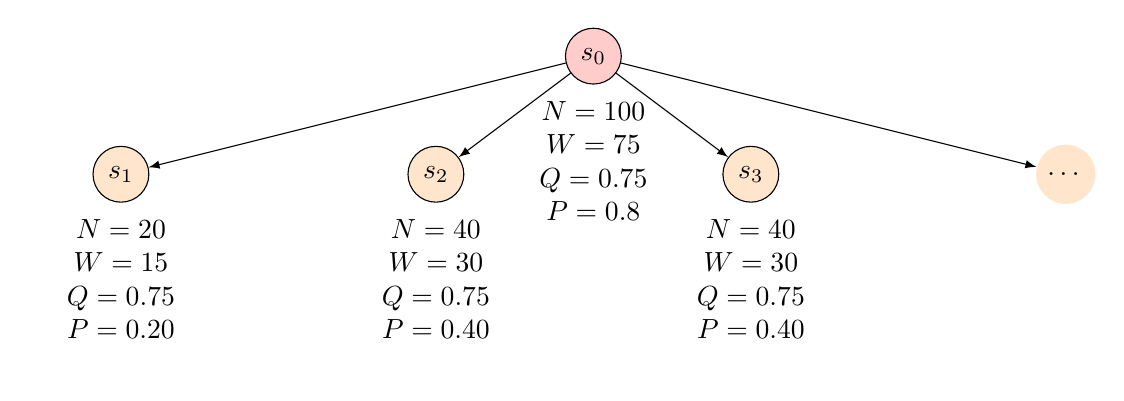
\begin{tikzpicture}[
      level 1/.style={sibling distance=40mm},
      level 2/.style={sibling distance=20mm},
      edge from parent/.style={draw,-latex},
      every node/.style={circle,draw,minimum size=7mm},
      label/.style={below=4pt, draw=none, fill=none, align=center}
      ]
      \node[label] {$N = 100$\\$W = 75$\\$Q = 0.75$\\$P = 0.8$} node[fill=red!20] {$s_0$}
        child {node[fill=orange!20] {$s_1$} node[label] {$N = 20$\\$W = 15$\\$Q = 0.75$\\$P = 0.20$}}
        child {node[fill=orange!20] {$s_2$} node[label] {$N = 40$\\$W = 30$\\$Q = 0.75$\\$P = 0.40$}}
        child {node[fill=orange!20] {$s_3$} node[label] {$N = 40$\\$W = 30$\\$Q = 0.75$\\$P = 0.40$}}
        child {node[fill=orange!20, draw=none] {$\dots$}};
    \end{tikzpicture}
    \caption{State-Action Pairs Storing a Set of Statistics}
    \label{fig:game-tree-with-stats}
\end{figure}

Each simulation begins at the root node of the search tree, $s_0$, and finishes when the simulation reaches a leaf node $s_L$ at time-step $L$, as shown in Figure \ref{fig:root-to-leaf}.

\begin{figure}[htb]
    \centering
    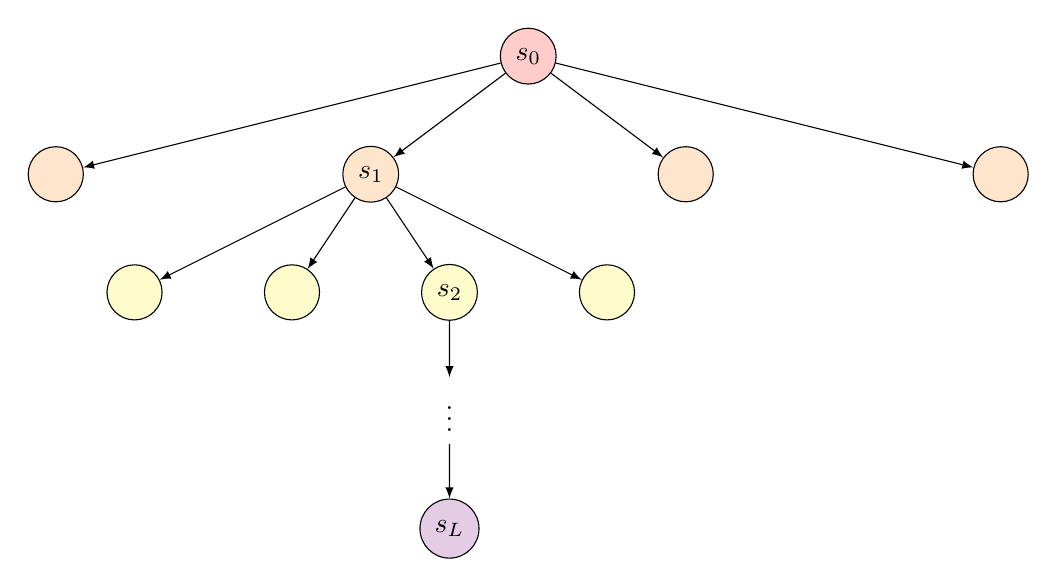
\begin{tikzpicture}[
      level 1/.style={sibling distance=40mm},
      level 2/.style={sibling distance=20mm},
      edge from parent/.style={draw,-latex},
      every node/.style={circle,draw,minimum size=7mm},
      label/.style={below=4pt, draw=none, fill=none, align=center}
      ]
      \node[fill=red!20] {$s_0$}
        child {node[fill=orange!20] {}}
        child {node[fill=orange!20] {$s_1$}
            child {node[fill=yellow!20] {}}
            child {node[fill=yellow!20] {}}
            child {node[fill=yellow!20] {$s_2$}
                child {node[draw=none] {$\vdots$}
                    child {node[fill=violet!20] {$s_L$}}}}
            child {node[fill=yellow!20] {}}}
        child {node[fill=orange!20] {}}
        child {node[fill=orange!20] {}};
    \end{tikzpicture}
    \caption{Simulation of MCTS on the Search Tree}
    \label{fig:root-to-leaf}
\end{figure}

At each of these time-steps, $t < L$, an action is selected $a_t = \operatorname{arg} \operatorname{max}_a \big(Q(s_t, a_t) + U(s_t, a_t)\big)$, using a variant of the Predictor + Upper-Confidence Bound Applied to Trees (PUCT) algorithm, $U(s, a) =  C(s) P(s, a) \sqrt{N(s)} / (1 + N(s, a))$, where $N(s)$ is the parent visit count and $C(s)$ is the exploration rate, which grows slowly with search time, $C(s) = \log\left((1 + N(s) + c_{base}) / c_{init}\right) + c_{init}$, but is essentially constant during the fast training games. The leaf node $s_L$ is added to a queue for neural network evaluation, $(\mathbf{p}, v) = f_\theta(s)$. The leaf node is expanded and each state-action pair $(s_L, a)$ is initialized to $\{N(s_L, a) = 0, W(s_L, a) = 0, Q(s_L, a) = 0, P(s_L, a) = p_a\}$. The visit counts and values are then updated in a backward pass through each step $t \leq L$, $N(s_t, a_t) = N(s_t, a_t) + 1$, $W(s_t, a_t) = W(s_t, a_t) + v$, $Q(s_t, a_t) = W(s_t,a_t) / N(s_t,a_t)$.

The modified Monte-Carlo Tree Search algorithm used in this paper is adapted from the AlphaZero framework. Internally, the node is represented as struct containing the current state and the action taken to get to this node, the index to its parent and the indices of its children, the prior policy of the node from the network, and the value and the number of visits of the node as shown in Listing \ref{lst:mcts_node}.

\begin{listing}[htb]
\begin{minted}[fontsize=\footnotesize]{cpp}
struct Node {
  using ID = std::int32_t;

  State state;
  Action action;

  Node::ID parent;
  std::vector<Node::ID> children;

  double prior = 0.0;
  double value = 0.0;
  double visits = 0.0;
};
\end{minted}
\caption{Node Representation for the Monte-Carlo Tree Search Algorithm}
\label{lst:mcts_node}
\end{listing}

The pseudocode for the modified Monte-Carlo Tree Search algorithm is shown in Algorithm \ref{alg:mcts}.

\begin{algorithm}[htb]
    \begin{algorithmic}[1]
        \Function{search}{state, model, simulations}
            \State root $\gets$ Node(state)
            \ForAll{$n \in \{1, 2,3, \ldots, \text{simulations}\}$}
                \State node $\gets$ root
        
                \Call{select}{node}
        
                \State optional\_terminal\_value $\gets$ game.terminal\_value(node.state, node.action)
                
                \If{optional\_terminal\_value.has\_value()}
                    \State value $\gets$ optional\_terminal\_value.value()
                \Else
                    \State value $\gets$ \Call{expand}{node, model}
                \EndIf
        
                \State \Call{backpropagate}{node, value}
            \EndFor

            \LComment{Action probability is proportional to child visits/}
            \State probs $\gets$ zero\_array(game.action\_size)
            \ForAll{i, child $\in$ root.children}
                \State probs[i] = child.visits
            \EndFor
            \State \Return probs / probs.sum()
        \EndFunction
    \end{algorithmic}
    \caption{Monte-Carlo Tree Search Algorithm}
    \label{alg:mcts}
\end{algorithm}

\clearpage

The pseudocode for \verb|select| function used in the modified Monte-Carlo Tree Search algorithm is shown in Algorithm \ref{alg:select}.

\begin{algorithm}[htb]
    \begin{algorithmic}[1]
        \Function{select}{node}
            \While{node.is\_expanded()}
                \State node $\gets$ \Call{highest\_child\_score}{node}
            \EndWhile
        \EndFunction
        
        \Function{highest\_child\_score}{node}
            \State child\_scores $\gets$ \{\}
            \ForAll{child $\in$ node.children}
                \State child\_scores.append(\Call{score}{child})
            \EndFor
            \Return \Call{max}{child\_scores}
        \EndFunction
        
        \Function{score}{node}
            \If{node.visits $>$ 0}
                \State mean $\gets \dfrac{1}{2}\cdot\left(\dfrac{ \text{node.value} }{ \text{node.visits} } + 1\right)$
                \If{node.parent.player $\neq$ node.player}
                    \State mean $\gets$ 1 $-$ mean
                \EndIf
            \Else
                \State mean $\gets$ 0
            \EndIf
            \State \Return $\text{mean} + \text{node.prior} \cdot C \cdot \dfrac{\sqrt{\text{node.parent.visits}}}{1 + \text{node.visits}}$  
        \EndFunction
    \end{algorithmic}
    \caption{Select Function for the Monte-Carlo Tree Search Algorithm}
    \label{alg:select}
\end{algorithm}

The pseudocode for \verb|expand| function used in the modified Monte-Carlo Tree Search algorithm is shown in Algorithm \ref{alg:expand}.

\begin{algorithm}[htb]
    \begin{algorithmic}[1]
        \Function{expand}{parent, model}
            \State legal\_actions $\gets$ game.legal\_actions(parent.state)
            \State policy, value $\gets$ model(game.encode\_state(parent.state))
            \State policy $\gets$ \Call{softmax}{policy}
            \State policy $\gets$ \Call{filter}{legal\_actions, policy}
            \State policy $\gets$ policy / policy.sum()
        
            \For{$i \in \{0, ..., \text{legal\_actions.size}\}$}
                \State legal\_actions $\gets$ legal\_actions[i]
                \State child\_state $\gets$ game.apply\_action(parent.state, action)
                \State prior $\gets$ policy[i]
                \State parent.children.append(Node(child\_state, action, prior))
            \EndFor
            \State \Return value
        \EndFunction
    \end{algorithmic}
    \caption{Expand Function for the Monte-Carlo Tree Search Algorithm}
    \label{alg:expand}
\end{algorithm}

The pseudocode for \verb|backpropagate| function used in the modified Monte-Carlo Tree Search algorithm is shown in Algorithm \ref{alg:backpropagate}.

\begin{algorithm}[htb]
    \begin{algorithmic}[1]
        \Function{backpropagate}{node, value}
            \While{node $\neq$ null}
                \State node.visits += 1
                \If{node.parent.state.player == node.state.player} 
                    \State node.value += value
                \Else
                    \State node.value -= value
                \EndIf
                \State node $\gets$ node.parent
            \EndWhile
        \EndFunction
    \end{algorithmic}
    \caption{Backpropagrate Function for the Monte-Carlo Tree Search Algorithm}
    \label{alg:backpropagate}
\end{algorithm}


The pseudocode for the  learning phase of the AlphaZero framework is shown in Algorithm \ref{alg:learning_phase}.

\begin{algorithm}[htb]
\begin{algorithmic}
    \Function{learn}{latest\_model, optimizer, iterations, selfplay\_iterations, training\_epochs}
        \For{$n \in \{0, \ldots, \text{iterations}\}$}
            \State memory $\gets$ \{\}

            \For{$i \in \{0, \ldots, \text{selfplay\_iterations}\}$}
                \State memory $+=$  \Call{self\_play}{latest\_model}
            \EndFor
            
            \For{$j \in \{0, \ldots, \text{training\_epochs}\}$}
                \State \Call{train}{latest\_model, memory, optimizer}
            \EndFor
        \EndFor
    \EndFunction
    \caption{Pseudocode for the Learning Phase of the AlphaZero Framework}
    \label{alg:learning_phase}
\end{algorithmic}
\end{algorithm}

\subsection{Self-Play}

The pseudocode for the  self-play data generation phase of the AlphaZero framework is shown in Algorithm \ref{alg:data-generation}.

\begin{algorithm}[htb]
    \begin{algorithmic}[1]
        \Function{self\_play}{model}
            \State history $\gets$ \{\}
            \State state $\gets$ game.initial\_state()
            \Loop
                \State probs $\gets$ \Call{search}{state, model}
                \State history.append((state, probs)) 
                \State action $\gets$ \Call{sample\_distribution}{probs}
                \State new\_state $\gets$ game.apply\_action(state, action)
                \State terminal\_value $\gets$ game.terminal\_value(new\_state)
                \If{terminal\_value.has\_value()}
                    \State memory $\gets$ \{\}
                    \ForAll{(hist\_state, hist\_probs) $\in$ history}
                        \State encoded $\gets$ game.encode\_state(hist\_state)
                        \State value $\gets$ hist\_state.player == player ? terminal\_value : -terminal\_value
                        \State memory.append((encoded, value, probs))
                    \EndFor
                    \State \Return memory
                \EndIf
                \State state $\gets$ new\_state
            \EndLoop
        \EndFunction
    \end{algorithmic}
    \caption{Pseudocode for the Self-Play Data Generation Phase of the AlphaZero Framework}
    \label{alg:data-generation}
\end{algorithm}


\subsection{Training}

The model is trained on the saved action probabilities as well as the outcome of playing that move which is saved on the \lstinline{memory} variable. 
    
\begin{algorithm}[htb]
\begin{algorithmic}
    \Function{train}{latest\_model, memory, optimizer}
        \State memory.shuffle()
        \For{$n \in \{0, \ldots, \text{iterations}\}$}
            \State feature, target\_value, target\_policy $\gets$ memory.sample\_batch()
            \State out\_value, out\_policy $\gets$ latest\_model(feature)
            \State loss $\gets$ \Call{mse\_loss}{out\_value, target\_value} +
            \Call{cross\_entropy}{out\_policy, target\_policy}
            \State optimizer.zero\_grad()
            \State loss.backward()
            \State optimizer.step()
        \EndFor
    \EndFunction
    \caption{Pseudocode for the Training Phase of the AlphaZero Framework}
    \label{alg:training_phase}
\end{algorithmic}
\end{algorithm}
\chapter{Results and Discussion}

\chapter{Conclusions and Recommendations} % ADVISER COMMENT (DON'T DELETE,2025-05-30): should be renamed to "Conclusions and Recommendations"

% Summary

The researchers were able to train a vision transformer model using the AlphaZero framework to learn how to play the game of Damath only through self-play. The model was able to learn and develop strategies without any prior knowledge and existing games between expert players, except for the rules of Damath.

The researchers were able to produce 5 different versions of the model, with the fifth and final version of the best model being able to beat the previous versions of the model and also beat an expert player in the game of Damath. 

After 100,000 games, the model rediscovered competent early game moves and discovered strategies that were discovered by Mr. Basanes. According to Mr. Basanes (\textit{personal communications}, May 23, 2025), the model was playing akin to a proficient player during the ten games that Mr. Basanes played against the model. The model demonstrates strong early game strategies but weak end-game moves throughout ten games.

% Findings

The researchers noticed that for most of the mid-to-late game states, the model gives a losing WDL prediction for both players and makes moves that lead to the model losing the game. This reflects the assessment of Mr. Basanes, wherein he states that the model demonstrates strong early game but weak middle-to-late game competence.

This shows that the model could not accurately predict the outcome and action probabilities of mid-to-late game states yet. This is more evident for earlier versions of the models, with WDL predictions and action priors becoming more accurate with newer versions of the model after a long amount of training time. This shows that a long amount of time is needed to train a model that can accurately predict the outcomes and action priors of various game states.

The outcome and action priors for early game states are much easier to predict as they are readily explored by the MCTS algorithm with varied outcomes. However, specific mid-to-late game configurations that might appear in a regular game between human players are less likely to be explored by the MCTS algorithm due to the branching factor of the game and the exploitative term of the PUCT algorithm. A higher number of MCTS simulations is needed for the PUCT algorithm to be able to use its exploratory term, which increases with the number of visits.

The model needs to train on more data of self-play games with a higher number of MCTS simulations to be able to accurately predict the outcome and action priors of various game states. With more data, the model will be able to generalize its predictions to all different kinds of game state that might appear on Damath. However, a relatively small amount of self-play game data is used for this study due to the limited computational resources compared to AlphaZero, where millions of self-play game data are used to beat a grandmaster in Chess and Go (\cite{silver2017masteringchessshogiselfplay}).

% \section{Recommendations}

Throughout this study, only 100,000 Damath games have been played in 20 iterations. However, the models by \cite{silver2017masteringchessshogiselfplay} were trained for 44 million games to master chess. The researchers recommend scaling the number of games during the generation of self-play data per iteration. Increasing the number of games produced per iteration should improve the model's competence in the game of Damath by allowing the model to learn through varied states of the game and their outcome, and thus having a more generalized understanding of the game.

The researchers also recommend increasing the number of MCTS simulations for each move during the self-play data generation phase of each iteration. This will allow the MCTS algorithm to better explore the game tree and assess legal actions through more varied game outcomes. Having more samples of the game outcomes for each move should let the MCTS algorithm better assess the probability of choosing an action leading to a favorable outcome, and letting the model learn through this policy should increase its competence.

The authors also recommend increasing parameters such as the number of transformer encoder blocks of the model as the vision transformer architecture improves the deeper the network goes, as shown by \cite{dosovitskiy2021imageworth16x16words}. Compared to convolutional neural networks that plateau as it trains longer, transformers keep on improving as it trains for the same amount of time. This is more evident for transformer with deeper encoder blocks. However, this would also increase the training time needed to minimize the training loss of the model.

The researchers recommend that the model learns through self-play data generated with random playout for the first initial moves as done by \cite{Popic_Boskovic_Brest_2021}. This ensures that the model explores all possible opening moves without the PUCT algorithm exploiting the winning opening sequences it initially finds. This should let the model accurately predict the outcome and action priors of various early game states and the following mid-to-late game states that might arise from the random early game state.

% The researchers recommend having the model train with temperature decreasing towards the end of the game as done by \cite{Popic_Boskovic_Brest_2021} to let the model explore other best moves randomly at the beginning of each game before playing deterministically towards the end of each game.

% ADVISER COMMENT (DON'T DELETE):
% 2025-05-21
% General Comments:
% -why did you only have 3 games against Mr. Basanes? it would be better to have more games to get a better gauge of the model's capabilities
% -MAJOR CONCERN: does Mr. Basanes know how the model works? this might give him an unfair advantage against the model
% -Methodology:
% --need to define the variables and what their values are
% -Results and Discussion
% --need to add more discussion to the results. results are just being presented and not discussed. Ex: what was the exploit that Mr. Basanes used and why did it

\bibliographystyle{apalike}
\bibliography{references}

\begin{appendices}

\chapter{Signed Letter of Informed Consent}

\begin{figure}[H]
    \centering
    \begin{subfigure}{0.3\textwidth}
        \centering
        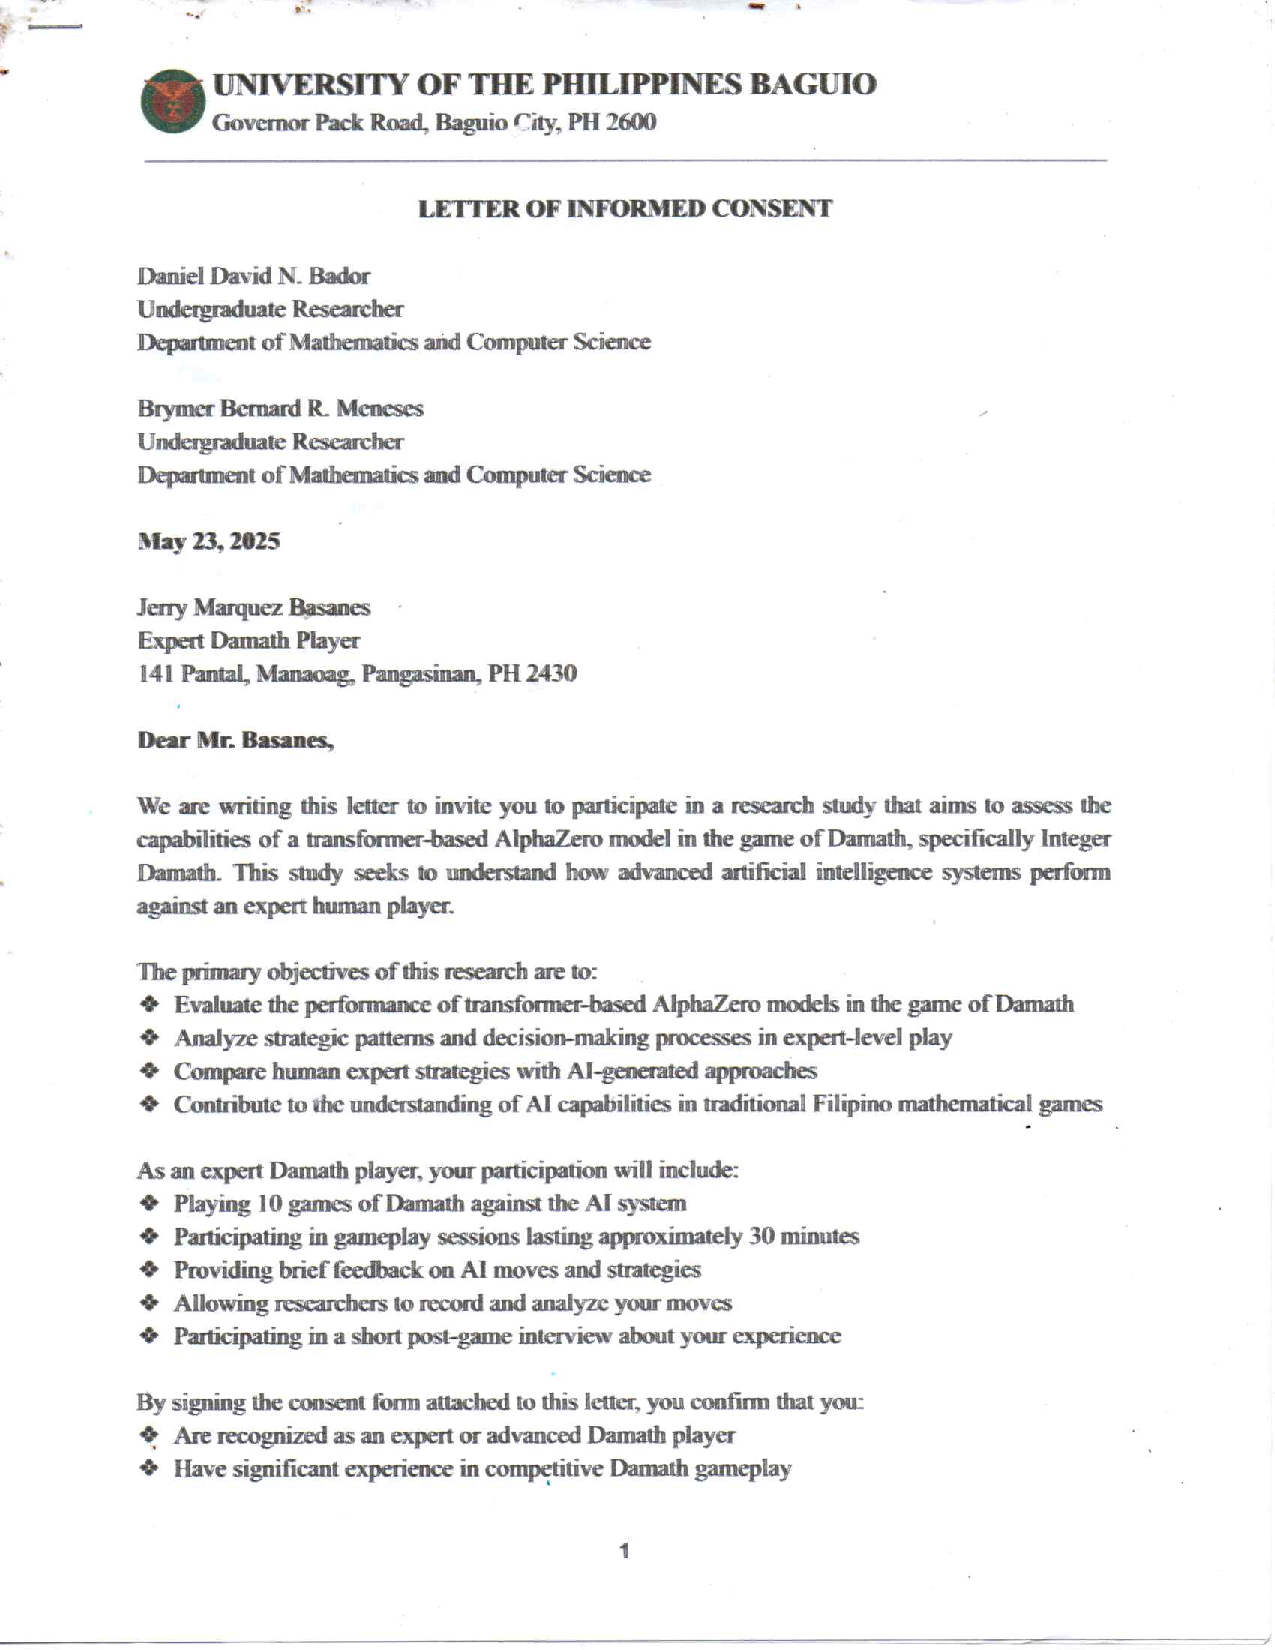
\includegraphics[page=1,width=\linewidth]{images/Letter of Informed Consent.pdf}
    \end{subfigure}
    \begin{subfigure}{0.3\textwidth}
        \centering
        \includegraphics[page=2,width=\linewidth]{images/Letter of Informed Consent.pdf}
    \end{subfigure}
    \begin{subfigure}{0.3\textwidth}
        \centering
        \includegraphics[page=3,width=\linewidth]{images/Letter of Informed Consent.pdf}
    \end{subfigure}
    \caption{Signed Letter of Informed Consent}
    \label{fig:signed-letter-of-informed-consent}
\end{figure}

\chapter{Games Against a Human Player}

\begingroup
\renewcommand\arraystretch{0.75}
\begin{longtable}[H]{cccccc}
    \hline
    \multicolumn{3}{c}{AI}       & \multicolumn{3}{c}{HUMAN}     \\ \hline
    Move         & Score & Total & Move          & Score & Total \\ \hline
      6 to (4,3) &      &  0    &   6 to (3, 4) &      &  0    \\ \hline
      6 to (5,4) &      &  0    &  -9 to (4, 3) & -15   & -15   \\ \hline
     -3 to (3,2) &      &  0    &  -9 to (2, 1) & -12   & -27   \\ \hline
                 &      &  0    &  -9 to (0, 3) &  81   &  54   \\ \hline
      0 to (1,2) &      &  0    &  -9 to (2, 1) &  -9    & 45    \\ \hline
    -11 to (3,2) &  99   &  99   &   6 to (2, 3) &      &  45    \\ \hline
    -11 to (1,4) &  $-5$  &  94  &  -1 to (0, 3) &  11   &  56    \\ \hline
     -1 to (6,3) &      &  94  &  10 to (4, 5) &      &  56    \\ \hline
      8 to (2,1) &      &  94  &  -1 to (1, 2) &      &  56    \\ \hline
      8 to (0,3) &  -8   &  86   &  -7 to (2, 5) &      &  56    \\ \hline
      8 to (1,4) &      &  86   &   4 to (2, 3) &  0.5  &  56.5  \\ \hline
     10 to (5,2) &      &  86   &  -3 to (6, 5) &      &  56.5  \\ \hline
     -1 to (7,4) &      &  86   &  10 to (3, 4) &      &  56.5   \\ \hline
     -1 to (5,6) &  -4   &  82   & -11 to (4, 5) &  11   &  67.5    \\ \hline
     -5 to (4,1) &      &  82   &   4 to (3, 2) &      &  67.5    \\ \hline
     -5 to (2,3) &  -1.25  &  80.75    &  10 to (1, 2) &  -2    &  65.5    \\ \hline
     10 to (4,3) &      &  80.75    &  -7 to (3, 4) &      &  65.5    \\ \hline
     10 to (2,5) &  3    &  83.75    &  10 to (2, 1) &      &  65.5    \\ \hline
     10 to (1,6) &      &  83.75    &   2 to (2, 5) &  12    &  77.5    \\ \hline
     -7 to (5,2) &      &  83.75    &   0 to (6, 5) &      &  77.5    \\ \hline
     -7 to (6,3) &      &  83.75    &  10 to (1, 0) &      &  77.5    \\ \hline
      2 to (6,1) &      &  83.75    &  10 to (5, 4) &      &  77.5    \\ \hline
      2 to (5,2) &      &  83.75    & -11 to (3, 4) &      &  77.5    \\ \hline
     -7 to (4,5) &  -140  &  -56.25  &                &      &  77.5    \\ \hline
     -7 to (2,3) &  $0.\overline{63}$   &  $-55.61\overline{36}$   &   2 to (3,4)  &  0    &  77.5    \\ \hline
     -7 to (4,5) &  -14    &   $-69.61\overline{36}$&  -5 to (3,6)  &      &  77.5    \\ \hline
     -7 to (2,7) &  1.4    &  $-68.21\overline{36}$   &   0 to (5,4)  &      &  77.5    \\ \hline
     -7 to (6,3) &  -14    & $-82.21\overline{36}$     &   8 to (3,6)  &      &  77.5    \\ \hline
     -7 to (2,7) &  -1.75    &  $-83.9\overline{36}$   &               &      &      \\ \hline\hline 
                 &           &  $-91.9\overline{63}$   &               &      & 77.5  \\ \hline 
    \caption{Game Moves of the First Game Against an Expert Damath Player}
    \label{tab:first-game}
\end{longtable}
\endgroup

\begin{table}[H]
    \centering
    \begin{tabular}{cccccc}
        \hline
        \multicolumn{3}{c}{HUMAN}        & \multicolumn{3}{c}{AI}     \\ \hline
        Move         & Score & Total & Move          & Score & Total \\ \hline
          -1 to (3,3) &      &  0    &   -9 to (5, 4) &      &  0    \\ \hline
          -1 to (6,5) & $0.\overline{1}$ &  $0.\overline{1}$  &    0 to (5, 4) & 0      &  0    \\ \hline
          4 to (5,3) &      & $0.\overline{1}$  &    0 to (7, 2) &  $-4$    &  $-4$    \\ \hline
          10 to (5,2) &      &  $0.\overline{1}$    &    -3 to (6, 5) &      &  $-4$    \\ \hline
          -5 to (4,1) &      &  $0.\overline{1}$    &    0 to (5, 0) &  0    &  $-4$    \\ \hline
          6 to (3,3) &      &  $0.\overline{1}$    &    0 to (3, 2) &  0    &  $-4$    \\ \hline
                     &      &  $0.\overline{1}$    &    0 to (5, 4) &  0    &  $-4$    \\ \hline
          10 to (5,3) &      &  $0.\overline{1}$    &    0 to (7, 2) &  $-20$    &  $-24$    \\ \hline
          2 to (6,1) &      &  $0.\overline{1}$    &    0 to (5, 0) &  $0$    &  $-24$    \\ \hline
          -9 to (1,3) &      &  $0.\overline{1}$    &    0 to (1, 4) &  $-18$    &  $-42$    \\ \hline
          0 to (1,2) &      &  $0.\overline{1}$    &    -11 to (5, 6) &      &  $-42$    \\ \hline
          8 to (4,1) &      &  $0.\overline{1}$    &    0 to (5, 0) &  $0$    &  $-42$    \\ \hline
          -3 to (3,2) &      &  $0.\overline{1}$    &    0 to (1, 3) &  $0$    &  $-42$    \\ \hline
                     &      &  $0.\overline{1}$    &    0 to (0, 1) &  $0$    &  $-42$    \\ \hline
          -11 to (2,1) &      &  $0.\overline{1}$    &    0 to (1, 2) &      &  $-42$    \\ \hline
          -11 to (0,3) &  0    &  $0.\overline{1}$    &    -3 to (7, 4) &      &  $-42$    \\ \hline
          -11 to (1,4) &      &  $0.\overline{1}$    &    4 to (2, 3) &  $-0.\overline{36}$    &  $-42.\overline{36}$    \\ \hline \hline
                       &     &   $0.\overline{1}$  &                &          &  $-39.\overline{36}$
    \end{tabular}
    \caption{Game Moves of the Second Game Against an Expert Damath Player}
    \label{tab:second-game}
\end{table}

\begin{table}[H]
    \centering
    \begin{tabular}{cccccc}
        \hline
        \multicolumn{3}{c}{AI}        & \multicolumn{3}{c}{HUMAN}     \\ \hline
        Move         & Score & Total & Move          & Score & Total \\ \hline
          6 to (4,3) &      &  0    &   6 to (3, 4) &      &  0    \\ \hline
          6 to (5,4) &      &  0    &   -9 to (4, 3) &  $-15$    &  $-15$    \\ \hline
          -3 to (3,2) &      &  0    &   -9 to (2, 1) &  $-12$    &  $-27$    \\ \hline
                      &      &  0    &   -9 to (0, 3) &  $81$    &  $54$    \\ \hline
          0 to (1,2) &      &  0    &   -9 to (2, 1) &  $-9$    &  $45$    \\ \hline
          -11 to (3,2) &  99  &  99    &   6 to (2, 3) &      &  $45$    \\ \hline
          -11 to (1,4) &  $-5$   &  94    &   -1 to (0, 3) &  $11$    &  $56$    \\ \hline
          10 to (3,2) &     &  94    &   -7 to (2, 5) &      &  $56$    \\ \hline
          4 to (6,3) &      &  94    &   10 to (4, 5) &      &  $56$    \\ \hline
          10 to (4,3) &      &  94    &   -7 to (3, 4) &      &  $56$    \\ \hline
          10 to (2,5) &  3    &  97    &   -3 to (6, 5) &      &  $56$    \\ \hline
          10 to (1,6) &      &  97    &   2 to (2, 5) &  $12$    &  $68$    \\ \hline
          8 to (4,1) &      &  97    &   -1 to (1, 2) &      &  $68$    \\ \hline
          4 to (7,4) &      &  97    &   -11 to (5, 6) &      &  $68$    \\ \hline
          -7 to (7,2) &      &  97    &   2 to (3, 4) &      &  $68$    \\ \hline
          8 to (3,2) &      &  97    &   2 to (2, 3) &      &  $68$    \\ \hline
          8 to (1,4) &  10    &  107    &   4 to (2, 3) &  $0.5$    &  $68.5$    \\ \hline
          -5 to (4,1) &      &  107    &   -1 to (2, 1) &      &  $68.5$    \\ \hline
          -1 to (4,3) &      &  107    &   10 to (3, 4) &      &  $68.5$    \\ \hline
          -1 to (2,5) &  9    &  116    &   -1 to (1, 0) &      &  $68.5$    \\ \hline
          -5 to (5,2) &      &  116    &   8 to (3, 6) &      &  $68.5$    \\ \hline
          -1 to (4,7) &  $-9$  & 107  0    &   -3 to (5, 4) &      &  $68.5$    \\ \hline
          -1 to (6,5) &  $0.\overline{18}$    & $107.\overline{18}$     &                &      &  $68.5$    \\ \hline
          -1 to (3,2) &  6    &  $113.\overline{18}$    &                &      &  $68.5$    \\ \hline
          -1 to (0,5) &  $-10$    &  $103.\overline{18}$    &   0 to (6,5)   &      &  $68.5$    \\ \hline
          4 to (5,6) &  $4$    &  $107.\overline{18}$    &   -1 to (6,5)   &      &  $68.5$    \\ \hline
          4 to (7,4) &  $-8$    &  $99.\overline{18}$   &   -5 to (1,6)   &      &  $68.5$    \\ \hline
          -1 to (2,7) &  $0.4$    & $99.5\overline{81}$     &                &      &  $68.5$    \\ \hline \hline
           &      & $91.5\overline{81}$     &                &      &  $68.5$    \\ \hline
    \end{tabular}
    \caption{Game Moves of the Third Game Against an Expert Damath Player}
    \label{tab:third-game}
\end{table}


\begin{table}[H]
    \centering
    \begin{tabular}{cccccc}
        \hline
        \multicolumn{3}{c}{AI}        & \multicolumn{3}{c}{HUMAN}     \\ \hline
        Move         & Score & Total & Move          & Score & Total \\ \hline
          -1 to (6,3) &      &  0    &   -1 to (1, 4) &      &  0    \\ \hline
          10 to (5,2) &      &  0    &   -9 to (5, 4) &      &  0    \\ \hline
          6 to (4,3) &      &  0    &   -9 to (3, 2) &  $-54$    &  $-54$    \\ \hline
          -3 to (4,3) &  6    &  6    &   6 to (3, 4) &      &  $-54$    \\ \hline
          -3 to (2,5) &  3    &  9    &               &      &  $-54$    \\ \hline
          -3 to (0,3) &  3    &  12    &   0 to (6,5)        &      &  $-54$    \\ \hline
          -1 to (7,4) &      &  12    &   -7 to (2,5)        &      &  $-54$    \\ \hline
          -3 to (1,4) &      &  12    &   -7 to (0,3)        &  21 &  $-33$    \\ \hline
                      &      &  12    &   -7 to (2,1)        &  $-16$    &  $-49$    \\ \hline
          -11 to (3,2) &  77    &  89    &   10 to (2,5)        &      &  $-49$    \\ \hline
          8 to (2,1) &      &  89    &   8 to (3,6)        &      &  $-49$    \\ \hline
          0 to (1,2) &      &  89    &   2 to (1,6)        &      &  $-49$    \\ \hline
          0 to (0,3) &      &  89    &   0 to (5,4)        &      &  $-49$    \\ \hline
          -11 to (4,3) &      &  89    &   0 to (3,2)        &  $0$    &  $-49$    \\ \hline
                       &      &  89    &   0 to (1,0)        &  8    &  $-41$    \\ \hline
          -1 to (6,5) &      &  89    &   0 to (7,6)        &  2    &  $-39$    \\ \hline
          0 to (1,4) &      &  89    &   10 to (0,3)        &  0    &  $-39$    \\ \hline
          4 to (6,3) &      &  89    &   10 to (1,2)        &      &  $-39$    \\ \hline
          10 to (4,3) &      &  89    &   0 to (2,1)        &  $20$    & $-19$      \\ \hline
          -7 to (5,2) &      &  89    &   0 to (4,3)        &      &  $-19$    \\ \hline
          -7 to (3,4) &  $-14$  & $75$      &   -3 to (4,5)        &     &  $-19$    \\ \hline
          -7 to (5,6) &  $-10$    &  65    &   -11 to (4,5)        &  77    &  58    \\ \hline
          4 to (7,4) &      &  65    &   10 to (0,1)        &      &  58    \\ \hline
          2 to (6,1) &      &  65    &   10 to (1,0)        &      &  58    \\ \hline
          2 to (7,2) &      &  65    &   2 to (2,5)        &      &  58    \\ \hline
          -5 to (4,1) &      &  65    &   2 to (3,4)        &      &  58    \\ \hline
          2 to (6,3) &      &  65    &   -11 to (5,4)        &      &  58    \\ \hline
          2 to (4,5) &  $-22$    &  43    &         &      &  58    \\ \hline
          2 to (2,3) &  1    &  44    &  4 to (1, 4)       &      &  58    \\ \hline
          2 to (0,5) &  $-2$    &  42    &  8 to (2, 5)       &      &  58    \\ \hline
          2 to (1,6) &      &  42    &  8 to (0, 7)       &  16    &  74    \\ \hline
          -5 to (3,2) &      &  42    &  10 to (7, 6)       &  30    &  104    \\ \hline
          4 to (6,5) &      &  42    &  10 to (3, 2)       &  80    &  184    \\ \hline\hline
                     &      &  42    &                     &     &  207    \\ \hline
    \end{tabular}
    \caption{Game Moves of the Fourth Game Against an Expert Damath Player}
    \label{tab:fourth-game}
\end{table}

\begin{table}[H]
    \centering
    \begin{tabular}{cccccc}
        \hline
        \multicolumn{3}{c}{AI}        & \multicolumn{3}{c}{HUMAN}     \\ \hline
        Move         & Score & Total & Move          & Score & Total \\ \hline
          -1 to (6,3) &     &  0    &   6 to (3, 4) &      &  0    \\ \hline
          6 to (2,3) &     &  0    &   10 to (4, 5) &      &  0    \\ \hline
          -1 to (5,4) &     &  0    &   -9 to (4, 3) & $-8$   &  $-8$    \\ \hline
          -3 to (3,2) &     &  0    &   -9 to (2, 1) & $-12$   &  $-20$    \\ \hline
                      &     &  0    &   -9 to (0, 3) & 81   &  $61$    \\ \hline
          0 to (1,2) &      &  0    &   -9 to (2, 1) & $-9$   &  $52$    \\ \hline
          -11 to (3,2) &  99 &  99    & 6 to (1, 2) & $1$   &  $53$    \\ \hline
          10 to (5,2) &   &  99       & 4 to (1, 4) &    &  $53$    \\ \hline
          10 to (6,3) &   &  99       & 4 to (2, 3) &    &  $53$    \\ \hline
          -11 to (1,4) & $-7$   &  92  &            &    &  $53$    \\ \hline
          -11 to (3,6) & $11$   &  103  &            &    &  $53$    \\ \hline
          -11 to (5,4) & $-1.1$   &  $101.9$  & 0 to (6,5)      &    &  $53$    \\ \hline
          -11 to (7,6) & $-11$   &  $90.9$  & 6 to (0,1)      &    &  $53$    \\ \hline
          10 to (7,4) &    &  $90.9$  & $-3$ to (4,5)      &    &  $53$    \\ \hline
          8 to (4,1) &    &  $90.9$  & $6$ to (1,0)      &    &  $53$    \\ \hline
          8 to (3,2) &    &  $90.9$  & $6$ to (5,4)      & 1.5    &  $54.5$    \\ \hline
          4 to (6,3) &    &  $90.9$  & $6$ to (7,2)      & 4    &  $58.5$    \\ \hline
          -5 to (4,1) &    &  $90.9$  & $6$ to (5,0)      & $-1.7143$  &  $56.7857$    \\ \hline
                      &    &  $90.9$  & $6$ to (0,5)      & 22  &  $78.7857$    \\ \hline
          2 to (6,1) &    &  $90.9$  & $8$ to (5,6)      &   &  $78.7857$    \\ \hline
          2 to (7,2) &    &  $90.9$  & $-3$ to (5,4)      &   &  $78.7857$    \\ \hline
          2 to (6,3) &    &  $90.9$  & $-3$ to (7,2)      & $-5$   &  $73.7857$    \\ \hline
          10 to (6,5) &    &  $90.9$  & $8$ to (7,4)      & $80$   &  $153.7857$    \\ \hline\hline
                      &    &  $79.9$  &                   &        &  $149.7857$    \\ \hline
    \end{tabular}
    \caption{Game Moves of the Fifth Game Against an Expert Damath Player}
    \label{tab:fifth-game}
\end{table}

\begin{table}[H]
    \centering
    \begin{tabular}{cccccc}
        \hline
        \multicolumn{3}{c}{AI}        & \multicolumn{3}{c}{HUMAN}     \\ \hline
        Move         & Score & Total & Move          & Score & Total \\ \hline
          -1 to (6,3) &      &  0    &   4 to (1, 4) &      &  0    \\ \hline
          -7 to (5,2) &      &  0    &   -1 to (3, 4) &      &  0    \\ \hline
          6 to (2,3) &       &  0    &   4 to (3, 2) &  24   &  24    \\ \hline
          -3 to (4,3) & $-7$ &  $-7$ &               &       &  24    \\ \hline
          -3 to (2,5) & $-4$ &  $-11$ &  -7 to (3,4) & $-4$ &  20    \\ \hline
          -7 to (4,3) &      &  $-11$ &  -7 to (5,2) & $-14$ &  6    \\ \hline
                      &      &  $-11$ &  -7 to (7,4) & $7$   &  13    \\ \hline
          2 to (6,1)  &      &  $-11$ &  -7 to (6,3) &       &  13    \\ \hline
          4 to (5,4)  & $-0.5714$  &  $-11.5714$ &  6 to (6,3) & 10       &  23    \\ \hline
          -11 to (2,1)  &          &  $-11.5714$ &  6 to (5,2) &          &  23    \\ \hline
          2 to (4,3)  & $-4$       &  $-15.5714$ &  $-9$ to (5,4) &          &  23    \\ \hline
          2 to (6,5)  & $-0.\overline{22}$    &  $-15.57937$ &  $0$ to (5,4) &  0 &  23    \\ \hline
          $-9$ to (2,3)  &    &  $-15.57937$ &  $-3$ to (6,5) &    &  23    \\ \hline
          $10$ to (5,2)  &    &  $-15.57937$ &  $0$ to (4,3) &    &  23    \\ \hline
          $10$ to (3,4)  & 10    &  $-5.57937$ &  $10$ to (4,5) &    &  23    \\ \hline
          $10$ to (5,6)  & 20    &  $14.2063$ &                 &    &  23    \\ \hline
          $10$ to (7,4)  & -30    &  $-15.7937$ & 8 to (5,6)    &    &  23    \\ \hline
          $-5$ to (4,1)  &        &  $-15.7937$ & $-11$ to (7,6) &    &  23    \\ \hline
          $-5$ to (5,2)  &        &  $-15.7937$ & $8$ to (6,5) &    &  23    \\ \hline
          $10$ to (5,6)  & 18     &  $2.2063$   & $-11$ to (6,5) &    &  23    \\ \hline
          $10$ to (7,4)  & -110   &  $-107.7937$ & $-5$ to (3,6) &    &  23    \\ \hline
          $10$ to (6,5)  &        &  $-107.7937$ & $-5$ to (4,5) &    &  23    \\ \hline
          $10$ to (7,6)  &        &  $-107.7937$ & $2$ to (1,6) &    &  23    \\ \hline
          $8$ to (4,1)  &        &  $-107.7937$ & $2$ to (0,5) &    &  23    \\ \hline
          $-9$ to (3,4)  &        &  $-107.7937$ & $-5$ to (2,3) & $0.\overline{5}$    &  $23.\overline5$   \\ \hline
          $0$ to (1,2)  &        &  $-107.7937$ & $-5$ to (0,1) & $-5$    &  $18.\overline5$   \\ \hline
          $10$ to (6,7) &        &  $-107.7937$ & $-5$ to (1,0) &         &  $18.\overline5$   \\ \hline
          $-5$ to (4,3) &        &  $-107.7937$ & $-5$ to (3,2) & $110$     &  $128.\overline5$   \\ \hline
                        &        &  $-107.7937$ & $-5$ to (7,6) & $0$       &  $128.\overline5$   \\ \hline
          $10$ to (4,5) &        &  $-107.7937$ & $-5$ to (3,2) &           &  $128.\overline5$   \\ \hline
          $8$ to (2,3) & $-3.2$  &  $-110.9937$ & $2$ to (1,4) &           &  $128.\overline5$   \\ \hline
          $8$ to (0,5) & 6       &  $-104.9937$ &              &           &  $128.\overline5$   \\ \hline \hline
                       &         &  $-76.9937$ &             &           &  $128.\overline5$   \\ \hline
    \end{tabular}
    \caption{Game Moves of the Sixth Game Against an Expert Damath Player}
    \label{tab:sixth-game}
\end{table}

\begin{table}[H]
    \centering
    \begin{tabular}{cccccc}
        \hline
        \multicolumn{3}{c}{HUMAN}        & \multicolumn{3}{c}{AI}     \\ \hline
        Move         & Score & Total & Move          & Score & Total \\ \hline
         $-1$ to (3,3) &       &  0    &   6 to (3, 4) &       &  0    \\ \hline
         $-7$ to (5,2) &       &  0    &   $-3$ to (4, 5) &       &  0    \\ \hline
         $-7$ to (5,3) &       &  0    &   $6$ to (5, 2) & $5$    &  5    \\ \hline
                       &       &  0    &   $6$ to (7, 4) & $-42$    &  $-37$  \\ \hline
         $6$ to (3,3)  &       &  0    &   $8$ to (5, 6) &        &  $-37$    \\ \hline
         $6$ to (5,4)  &       &  0    &   $-3$ to (5, 3) & $3$    &  $-34$    \\ \hline
         $4$ to (5,4)  & $-1.\overline3$ &  $-1.\overline3$   &   $-9$ to (3, 3) & $-13$    &  $-47$    \\ \hline
         $-3$ to (3,2)  &       &  $-1.\overline3$    &   $-9$ to (2, 1) & $-12$    &  $-59$    \\ \hline
                        &       &  $-1.\overline3$    &   $-9$ to (0, 3) & $81$    &  $22$    \\ \hline
         $0$ to (1,2)  &       &  $-1.\overline3$     &   $-9$ to (2, 1) & $-9$    &  $13$    \\ \hline
         $-11$ to (3,2)  &   99 &  $97.\overline6$     &   $0$ to (6, 5) &         &  $13$    \\ \hline
         $10$ to (5,2)  &       &  $97.\overline6$     &   $-1$ to (3, 4) &         &  $13$    \\ \hline
         $-11$ to (1,3)  &       &  $97.\overline6$     &   $-1$ to (1, 2) & $0.\overline{09}$ &  $13.\overline{09}$    \\ \hline
         $8$ to (2,1)  &       &  $97.\overline6$     &   $-1$ to (3, 0) & $-9$ &  $4.\overline{09}$    \\ \hline
         $2$ to (6,1)  &       &  $97.\overline6$     &   $-1$ to (5, 3) & $18$ &  $22.\overline{09}$    \\ \hline
         $-5$ to (4,1)  &       &  $97.\overline6$     &   $-1$ to (3, 0) & 8 &  $30.\overline{09}$    \\ \hline
         $2$ to (5,2)  &        &  $97.\overline6$     &   $-1$ to (5, 3) & 2 &  $32.\overline{09}$    \\ \hline \hline
                       &        &  $97.\overline6$     &                  &   &  $37.\overline{09}$    \\ \hline
    \end{tabular}
    \caption{Game Moves of the Seventh Game Against an Expert Damath Player}
    \label{tab:seventh-game}
\end{table}

\begin{table}[H]
    \centering
    \begin{tabular}{cccccc}
        \hline
        \multicolumn{3}{c}{HUMAN}        & \multicolumn{3}{c}{AI}     \\ \hline
        Move         & Score & Total & Move          & Score & Total \\ \hline
          6 to (3,3) &       &  0    &   6 to (5, 4) &       &  0    \\ \hline
          10 to (3,2) &       &  0    &   6 to (5, 3) &       &  0    \\ \hline
          4 to (5,4) & $0.\overline6$ &  $0.\overline6$    &   $-5$ to (7, 4) &       &  0    \\ \hline
          $-1$ to (5,3) &             &  $0.\overline6$    &   $-9$ to (5, 2) & $-10$       &  $-10$    \\ \hline
                        &             &  $0.\overline6$    &   $-9$ to (3, 4) & $-15$       &  $-25$    \\ \hline
          $-9$ to (1,3) &             &  $0.\overline6$    &   $-9$ to (1, 2) & $1$       &  $-24$    \\ \hline
          $-3$ to (0,3) & $27$        &  $27.\overline6$    &   $0$ to (6, 5) &           &  $-24$    \\ \hline
          $4$ to (7,6)  & $4$        &  $31.\overline6$     &   $10$ to (4, 5) &           &  $-24$    \\ \hline
          $-7$ to (5,2)  &          &  $31.\overline6$     &   $8$ to (3, 6) &           &  $-24$    \\ \hline
          $0$ to (1,2)  &           &  $31.\overline6$     &   $-1$ to (3, 4) &           &  $-24$    \\ \hline
          $-7$ to (3,3)  &           &  $31.\overline6$     &   $-1$ to (5, 2) & $-8$           &  $-32$    \\ \hline
          $2$ to (6,1)  &           &  $31.\overline6$     &   $-1$ to (7, 0) & $-2$           &  $-34$    \\ \hline
          $10$ to (3,3)  &          &  $31.\overline6$     &   $-1$ to (3, 4) & $-22$           &  $-56$    \\ \hline
                         &          &  $31.\overline6$     &   $-1$ to (0, 1) & $-2$           &  $-58$    \\ \hline
          $-3$ to (1,4)  &          &  $31.\overline6$     &   $4$ to (1, 3) & $-1.\overline3$    &  $-59.\overline3$    \\ \hline
          $8$ to (2,1)  &          &  $31.\overline6$     &   $10$ to (3, 4) &                    &  $-59.\overline3$    \\ \hline
          $-5$ to (4,1)  &          &  $31.\overline6$     &   $-3$ to (6, 5) &                    &  $-59.\overline3$    \\ \hline
          $4$ to (5,4)  & $-1.\overline3$  &  $30.\overline3$    &   $-11$ to (5, 6) &                    &  $-59.\overline3$    \\ \hline
          $4$ to (6,5)  &                  &  $30.\overline3$    &   $-11$ to (7, 4) & $-44$                    &  $-103.\overline3$    \\ \hline
          $-5$ to (3,2)  &                  &  $30.\overline3$    &   $4$ to (4, 1) & $-20$                    &  $-123.\overline3$    \\ \hline
          $8$ to (1,2)  &                  &  $30.\overline3$    &   $-1$ to (1, 3) & $-0.25$                    &  $-123.58\overline3$    \\ \hline
          $-11$ to (0,1)  &                  &  $30.\overline3$    &   $-1$ to (0, 5) &                            &  $-123.58\overline3$    \\ \hline
          $-11$ to (1,2)  &                  &  $30.\overline3$    &   $-1$ to (1, 3) &                            &  $-123.58\overline3$    \\ \hline
          $-11$ to (0,3)  &                  &  $30.\overline3$    &   $-7$ to (1, 4) &                            &  $-123.58\overline3$    \\ \hline
          $-11$ to (1,4)  &                  &  $30.\overline3$    &   $4$ to (3, 0) &                            &  $-123.58\overline3$    \\ \hline
          $-11$ to (3,2)  & $22$                  &  $52.\overline3$    &   $4$ to (2, 1) &                            &  $-123.58\overline3$    \\ \hline
          $-11$ to (1,0)  & $-14$                  &  $38.\overline3$    &   $-11$ to (5, 3) &                            &  $-123.58\overline3$    \\ \hline
          $-11$ to (2,1)  &                        &  $38.\overline3$    &   $-11$ to (7, 2) &                            &  $-123.58\overline3$    \\ \hline
          $-11$ to (3,2)  &                        &  $38.\overline3$    &   $10$ to (3, 3) &                            &  $-123.58\overline3$    \\ \hline
          $-11$ to (5,4)  & $-1.1$                        &  $37.2\overline3$    &   $8$ to (4, 5) &                            &  $-123.58\overline3$    \\ \hline
          $-11$ to (3,6)  & $-88$                        &  $-50.7\overline6$    &   $-5$ to (4, 5) &            $55$ &  $-68.58\overline3$    \\ \hline \hline
                          &                              &  $-50.7\overline6$    &                  &           &  $-89.58\overline3$    \\ \hline \hline
    \end{tabular}
    \caption{Game Moves of the Eighth Game Against an Expert Damath Player}
    \label{tab:eighth-game}
\end{table}

\begin{table}[H]
    \centering
    \begin{tabular}{cccccc}
        \hline
        \multicolumn{3}{c}{HUMAN}        & \multicolumn{3}{c}{AI}     \\ \hline
        Move         & Score & Total & Move          & Score & Total \\ \hline
          $-9$ to (0,3) &                 &  0    &   $-1$ to (1, 4) &       &  0    \\ \hline
          $-9$ to (2,5) & $-10$           &  $-10$ &   $10$ to (1, 4) & $1$  &  $1$    \\ \hline
          $6$ to (3,3)  &                 &  $-10$ &   $-9$ to (5, 4) &      &  $1$    \\ \hline
          $6$ to (6,5)  & $-0.\overline6$ &  $-10.\overline6$ &   $0$ to (5, 4) & $0$      &  $1$    \\ \hline
          $4$ to (5,3)  &                 &  $-10.\overline6$ &   $0$ to (7, 2) & $-4$      &  $-3$    \\ \hline
          $10$ to (3,2)  &                &  $-10.\overline6$ &   $-11$ to (7, 6) &           &  $-3$    \\ \hline
          $0$ to (1,2)  &                &  $-10.\overline6$ &   $10$ to (0, 3) &           &  $-3$    \\ \hline
          $-5$ to (4,1)  &                &  $-10.\overline6$ &   $0$ to (5, 0) & $0$        &  $-3$    \\ \hline
          $10$ to (3,3)  &                &  $-10.\overline6$ &   $0$ to (3, 2) & $0$        &  $-3$    \\ \hline
                         &                &  $-10.\overline6$ &   $0$ to (5, 4) & $0$        &  $-3$    \\ \hline
          $-1$ to (5,3)  &                &  $-10.\overline6$ &   $0$ to (7, 2) & $2$        &  $-1$    \\ \hline
          $2$ to (6,1)  &                &  $-10.\overline6$ &   $0$ to (5, 0) & $0$        &  $-1$    \\ \hline
          $0$ to (1,3)  &                &  $-10.\overline6$ &   $0$ to (1, 4) & $0$        &  $-1$    \\ \hline
          $-3$ to (1,2)  &                &  $-10.\overline6$ &   $10$ to (2, 1) & $7$        &  $6$    \\ \hline
          $8$ to (1,2)  & $0.8$           &  $-9.8\overline6$ &   $0$ to (5, 0) &            &  $6$    \\ \hline
          $8$ to (0,3)  &                 &  $-9.8\overline6$ &   $0$ to (4, 1) &            &  $6$    \\ \hline
          $-11$ to (0,1)  &               &  $-9.8\overline6$ &   $0$ to (5, 3) &            &  $6$    \\ \hline
          $8$ to (1,4)  &                  &  $-9.8\overline6$ &   $4$ to (1, 3) & $0.5$      &  $6.5$    \\ \hline
          $-11$ to (1,2)  &                &  $-9.8\overline6$ &   $4$ to (0, 1) & $15$      &  $21.5$    \\ \hline \hline
                          &                &  $-9.8\overline6$ &                 &           &  $15.5$    \\ \hline \hline
    \end{tabular}
    \caption{Game Moves of the Ninth Game Against an Expert Damath Player}
    \label{tab:ninth-game}
\end{table}

\begin{table}[H]
    \centering
    \begin{tabular}{cccccc}
        \hline
        \multicolumn{3}{c}{HUMAN}        & \multicolumn{3}{c}{AI}     \\ \hline
        Move         & Score & Total & Move          & Score & Total \\ \hline
          4 to (5,3) &       &  0    &   6 to (3, 4) &       &  0    \\ \hline
          4 to (5,4) &       &  0    &   $-5$ to (3, 3) & $-13$       &  $-13$    \\ \hline
          6 to (5,4) & $-0.\overline6$  &  $-0.\overline6$  & $6$ to (1, 3) &        &  $-13$    \\ \hline
          $-9$ to (3,4) & $-15$  &  $-15.\overline6$  & $-1$ to (3, 3) & $8$        &  $-5$    \\ \hline
                        &        &  $-15.\overline6$  & $-1$ to (6, 5) & $-0.1\overline6$        &  $-5.1\overline6$    \\ \hline
          $10$ to (3,2) &        &  $-15.\overline6$  & $10$ to (4, 5) &            &  $-5.1\overline6$    \\ \hline
          $-7$ to (7,2) &        &  $-15.\overline6$  & $8$ to (3, 6) &            &  $-5.1\overline6$    \\ \hline
          $0$ to (1,2) &          &  $-15.\overline6$  & $8$ to (2, 5) &            &  $-5.1\overline6$    \\ \hline
          $0$ to (0,3) &          &  $-15.\overline6$  & $-1$ to (5, 4) &           &  $-5.1\overline6$    \\ \hline
          $-7$ to (5,3) &          &  $-15.\overline6$  & $-1$ to (7, 2) & $6$           &  $0.8\overline3$    \\ \hline
          $2$ to (6,1) &          &  $-15.\overline6$  & $4$ to (1, 4) &               &  $0.8\overline3$    \\ \hline
          $-3$ to (1,2) &          &  $-15.\overline6$  & $0$ to (6, 5) &               &  $0.8\overline3$    \\ \hline
          $-5$ to (4,1) &          &  $-15.\overline6$  & $-1$ to (5, 0) & $-0.5$       &  $0.\overline3$    \\ \hline
          $-11$ to (2,1) &         &  $-15.\overline6$  & $-1$ to (6, 1) &              &  $0.\overline3$    \\ \hline
          $-1$ to (7,0) & 2        &  $-13.\overline6$  & $-7$ to (0, 5) &              &  $0.\overline3$    \\ \hline
          $-5$ to (5,2) &          &  $-13.\overline6$  & $-11$ to (7, 6) &              &  $0.\overline3$    \\ \hline
          $10$ to (1,3) &          &  $-13.\overline6$  & $4$ to (3, 2) & $40$            &  $40.\overline3$    \\ \hline
                        &          &  $-13.\overline6$  & $4$ to (1, 0) & $-7$             &  $33.\overline3$    \\ \hline
          $8$ to (2,1) &          &  $-13.\overline6$  & $4$ to (3, 3) & $-8$          &  $25.\overline3$    \\ \hline
                       &          &  $-13.\overline6$  & $4$ to (6, 1) & $-1.6$          &  $23.7\overline3$    \\ \hline
          $-1$ to (5,2) & $6$     &  $-7.\overline6$  & $-5$ to (3, 6) &               &  $23.7\overline3$    \\ \hline
          $-3$ to (1,3) &         &  $-7.\overline6$  & $10$ to (5, 4) &               &  $23.7\overline3$    \\ \hline
          $-1$ to (3,3) &         &  $-7.\overline6$  & $10$ to (3, 2) & $-10$           &  $13.7\overline3$    \\ \hline
                        &         &  $-7.\overline6$  & $10$ to (1, 4) & $7$              &  $20.7\overline3$    \\ \hline \hline
                        &         &  $-7.\overline6$  &                &                  &  $14.7\overline3$    \\ \hline
    \end{tabular}
    \caption{Game Moves of the Tenth Game Against an Expert Damath Player}
    \label{tab:tenth-game}
\end{table}
\end{appendices}


\end{document}
